When studying temporal structures in neural dynamics, the definition of the time references is a key first point. In the computational analysis in the previous section, the time reference to define the intervals where first and last spike in the burts. In that case, as well as in the case of inter-neurons in \textit{C. maenas} the CPG phases are directly related with the bursting activity of these neurons. However, in the case of \textit{Lymnaea stagnalis}, activity is usually characterized using recordings from both inter-neurons and moto-neurons \parencite{elliot, benjamin, crossley}. This leads to a more flexible reference of the time references, so for this analysis, references will be defined by the phase and each phase will be bounded by different neurons. For example, in Figure \ref{fig:example lymnaea phases recording} the three phases in the  CPG are marked over the recording, note how it can be delimited by the neurons in the circuit but some of the moto-neurons cover several phases and that phases are delimited not only by the spikes but the hyperpolarization periods. Therefore, to characterize the time sequences in the feeding CPG, we need compound reference from several neural recordings that can be summarized as in Table \ref{table:cpg ref intervals}

%\TODO revisar
Table \ref{table:tabla spikes} displays a summary of some neurons involved in each phase. \todo{viene del tfm revisar}

% Please add the following required packages to your document preamble:
% \usepackage{multirow}
\begin{table}[htb!]
	\begin{tabular}{cl|l|ll}
		\multicolumn{1}{l}{}                                 & \multicolumn{1}{c|}{\textbf{N1}} & \multicolumn{1}{c|}{\textbf{N2}} & \multicolumn{1}{c}{\textbf{N3}} &  \\
		\multicolumn{1}{c|}{\multirow{2}{*}{\textbf{Start}}} & Last spike of N3t/B3             & Inhibition of B5                 & First spike of B8               &  \\
		\multicolumn{1}{c|}{}                                & Depolarization in B1             &                                  &                                 &  \\ \cline{1-4}
		\multicolumn{1}{c|}{\multirow{2}{*}{\textbf{End}}}   & Last spike of B5                 & First spike of B8                & Last spike of N3t/B3            &  \\
		\multicolumn{1}{c|}{}                                & Hyperpolarization in B1          &                                  &                                 & 
	\end{tabular}
	\caption{Time reference boundaries for the three phases in the feeding CPG}
	\label{table:cpg ref intervals}
\end{table}


\begin{table}[h!]
	\centering
	\begin{tabular}{lccc}
		Neuron                                           & \multicolumn{1}{l}{Protraction} & \multicolumn{1}{l}{Rasp} & \multicolumn{1}{l}{Swallow} \\ \hline
		Interneuron                                     & N1                              & N2                       & N3                          \\
		& \multicolumn{1}{l}{}            & \multicolumn{1}{l}{}     & \multicolumn{1}{l}{}        \\
		\multicolumn{1}{c}{\multirow{3}{*}{Motoneuron}} & B7                              & B10                      & B3                        \\
		\multicolumn{1}{c}{}                            & B6                              & B4                       & B9                        \\
		\multicolumn{1}{c}{}                            & B1                              &                          &                         
	\end{tabular}
	\caption{Neuron participation in feeding phases.}
	\label{table:tabla spikes}
\end{table}



\begin{figure}[bth!]
\centering
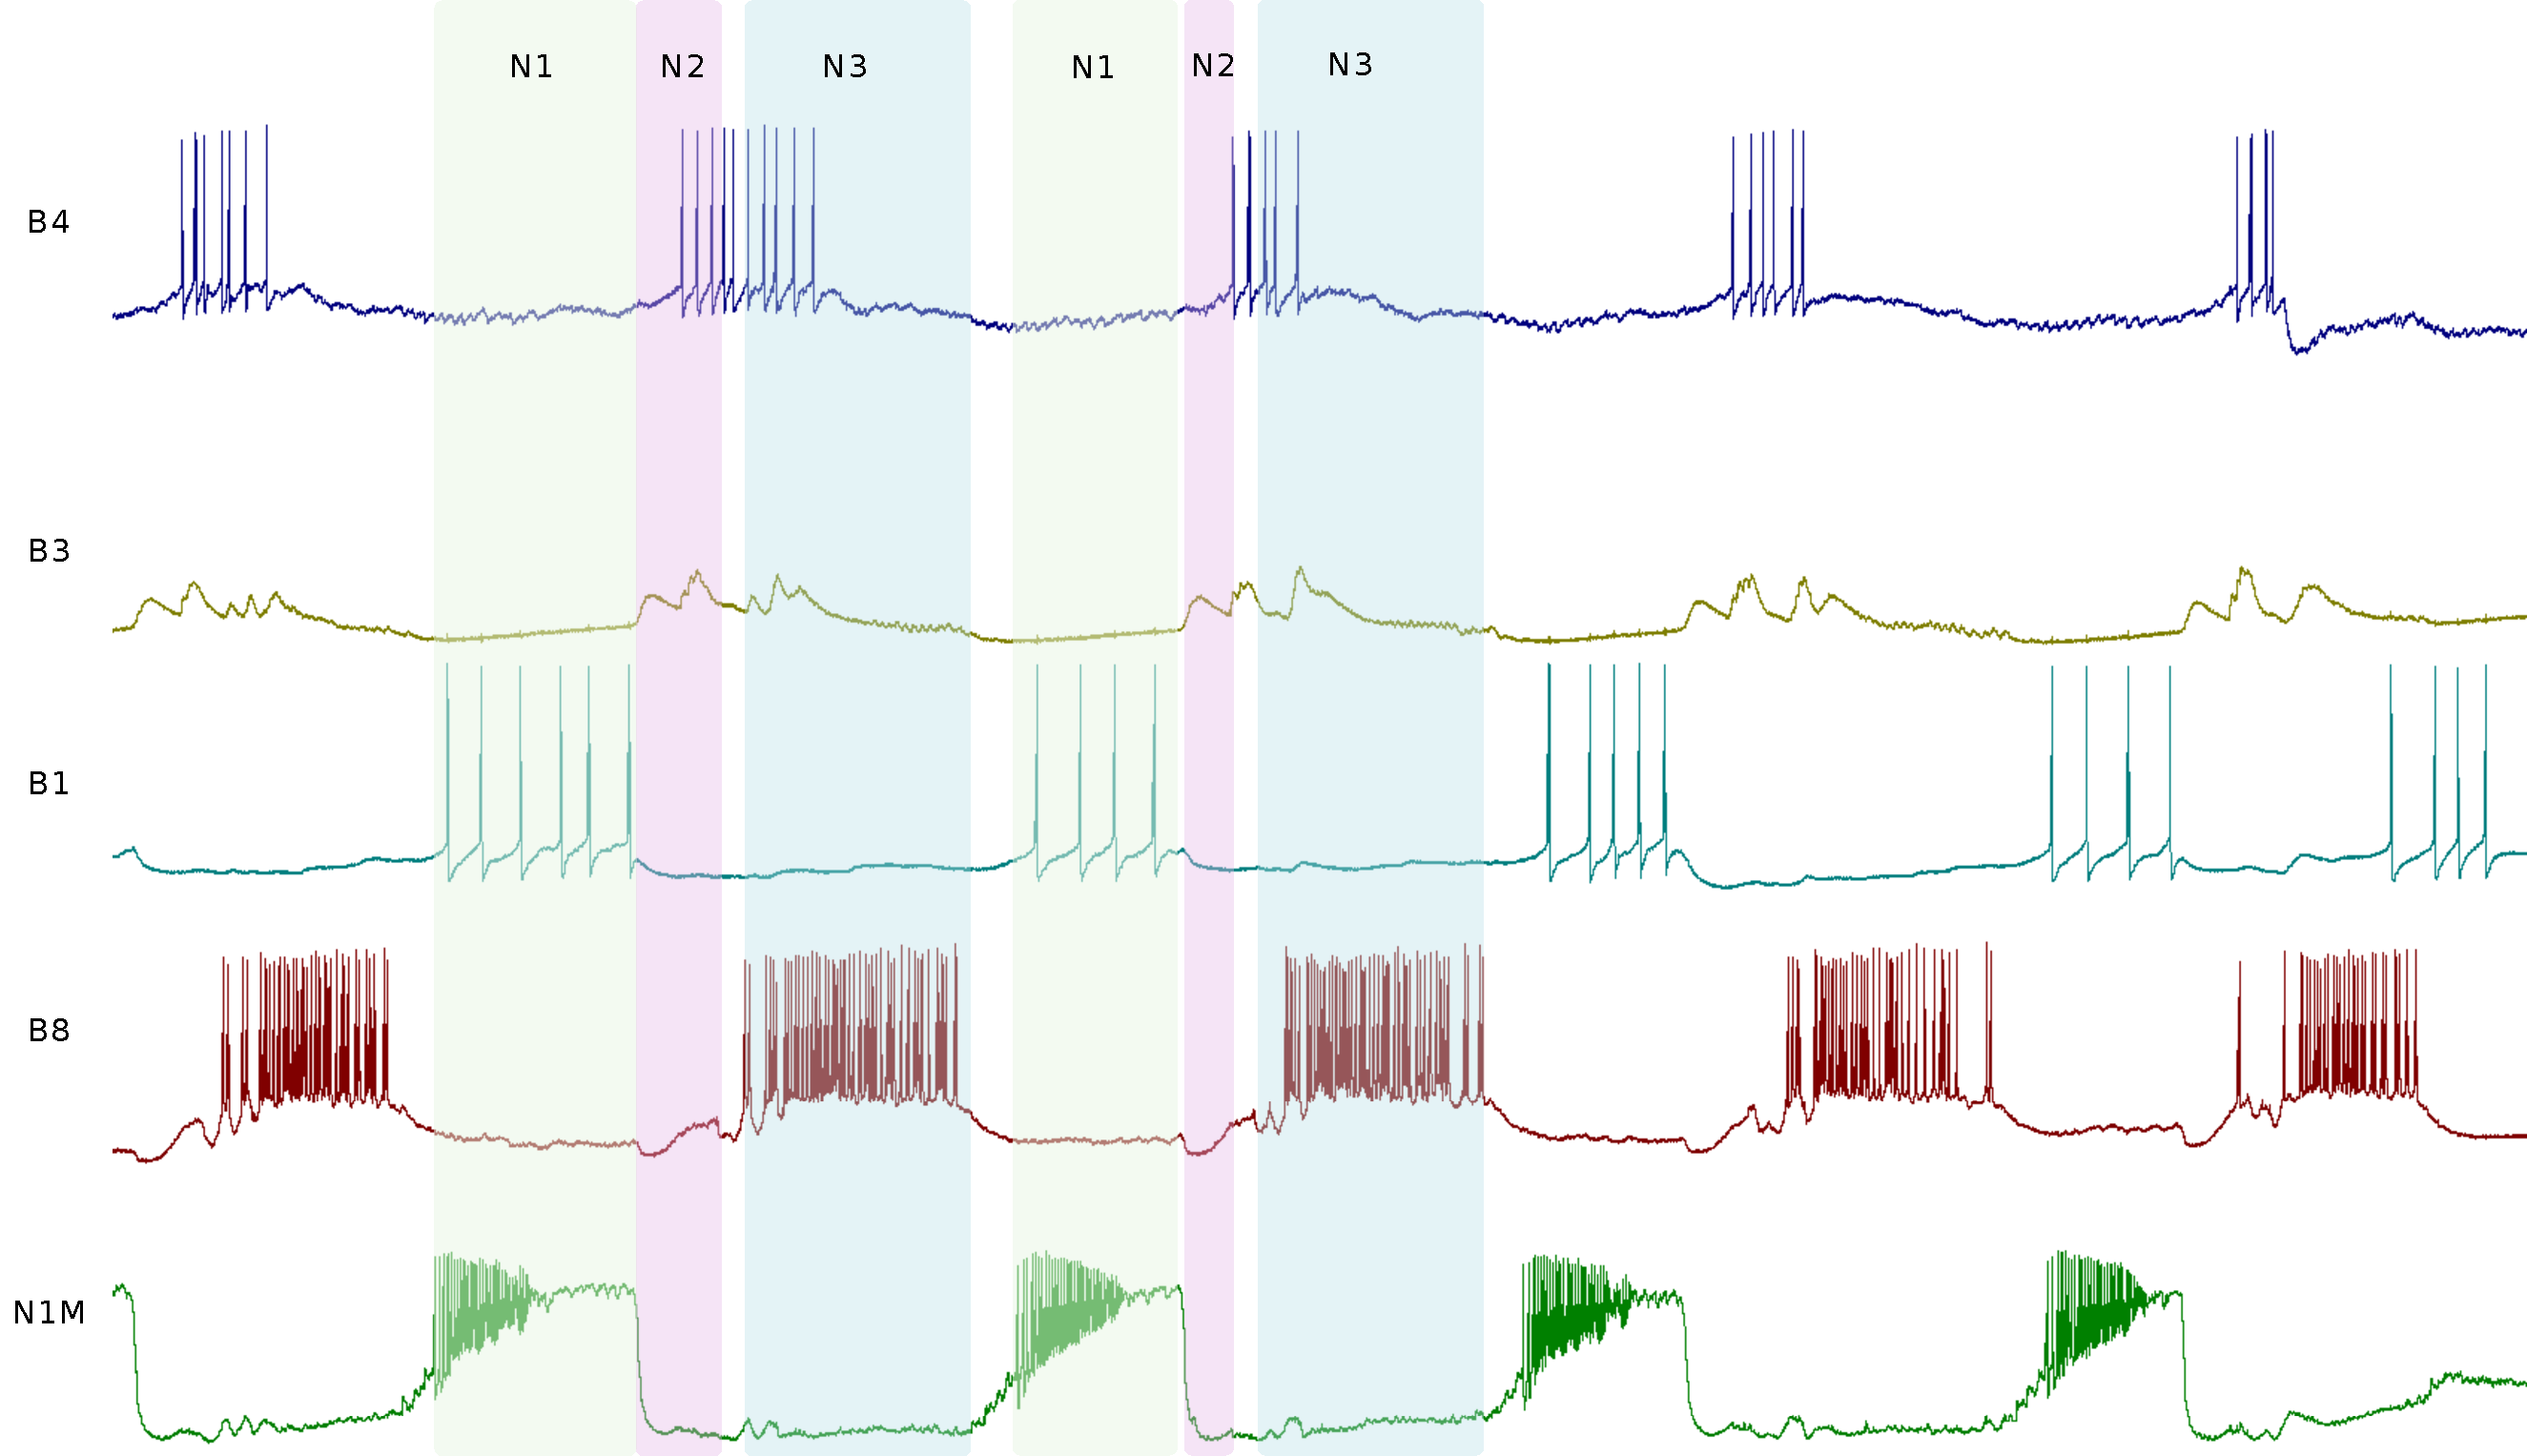
\includegraphics[width=\textwidth]{img/invariants/example_phases_1.pdf}
\\
\vspace{10pt}
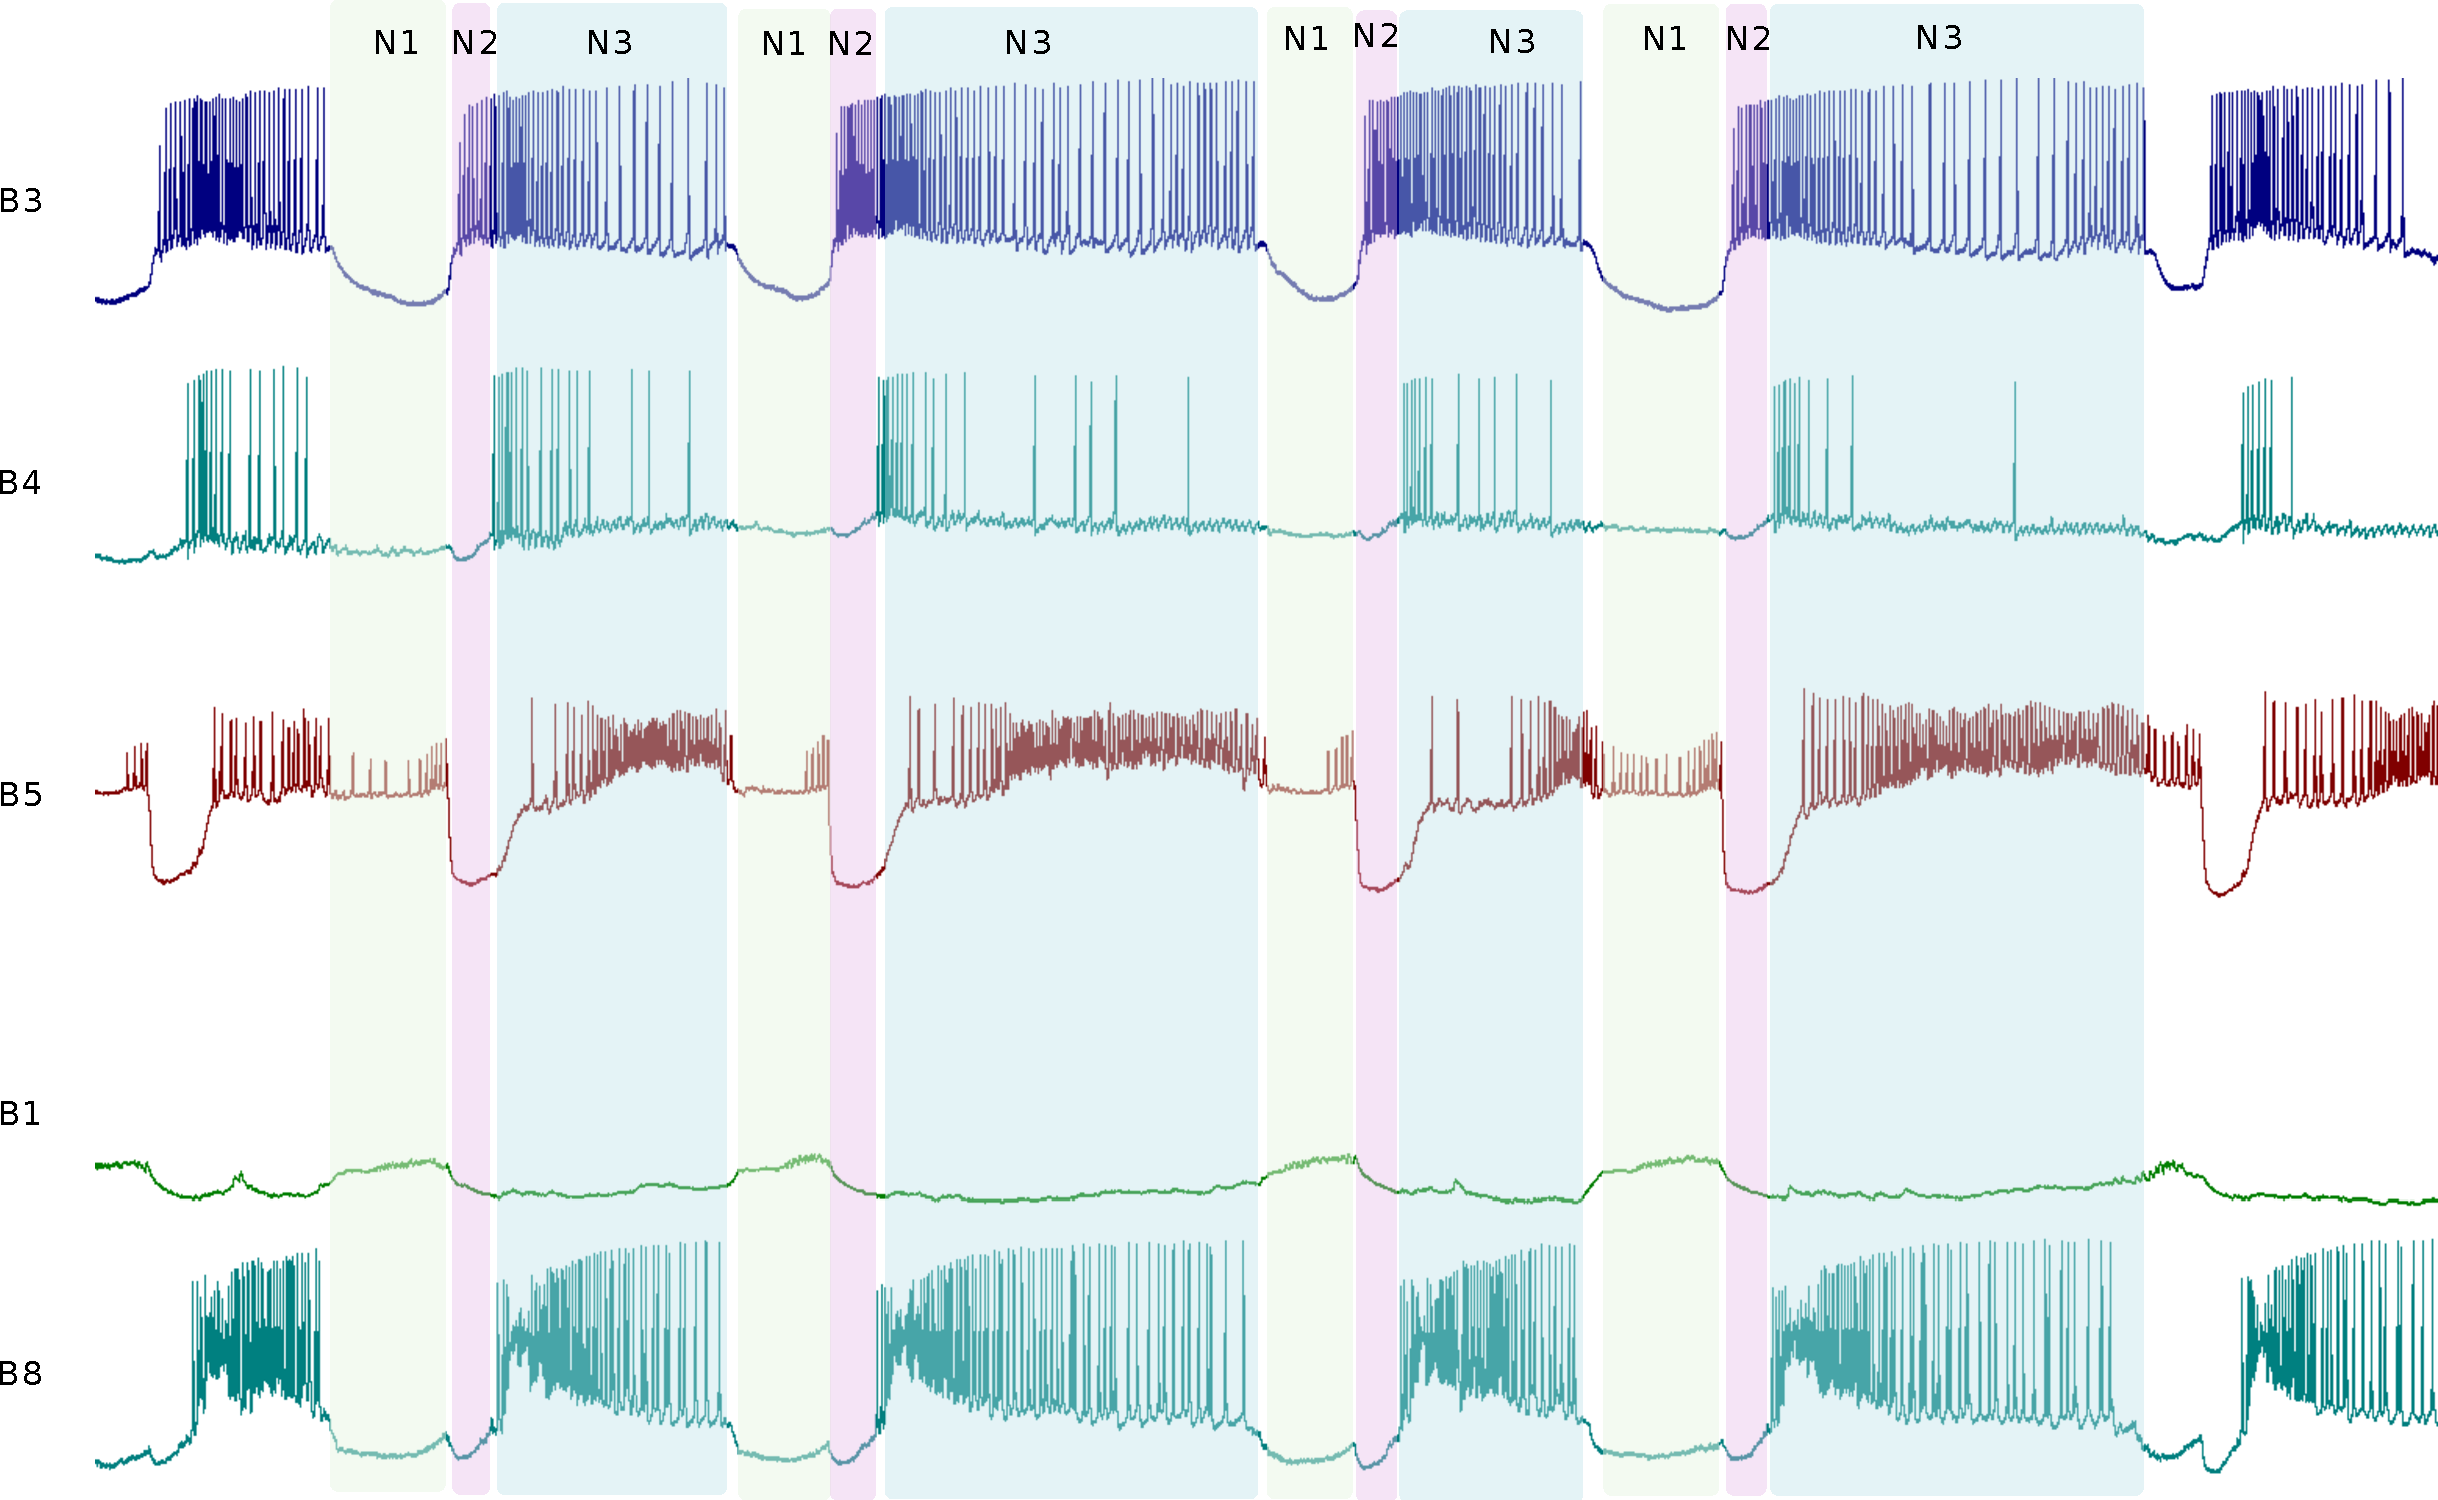
\includegraphics[width=\textwidth]{img/invariants/example_phases_2.pdf}
\caption{Delimitation of phases in the feeding CPG of \textit{Lymnaea stagnalis} based on different recordings.}
\label{fig:example lymnaea phases recording}
\end{figure}




\begin{figure}[bth!]
	\centering
	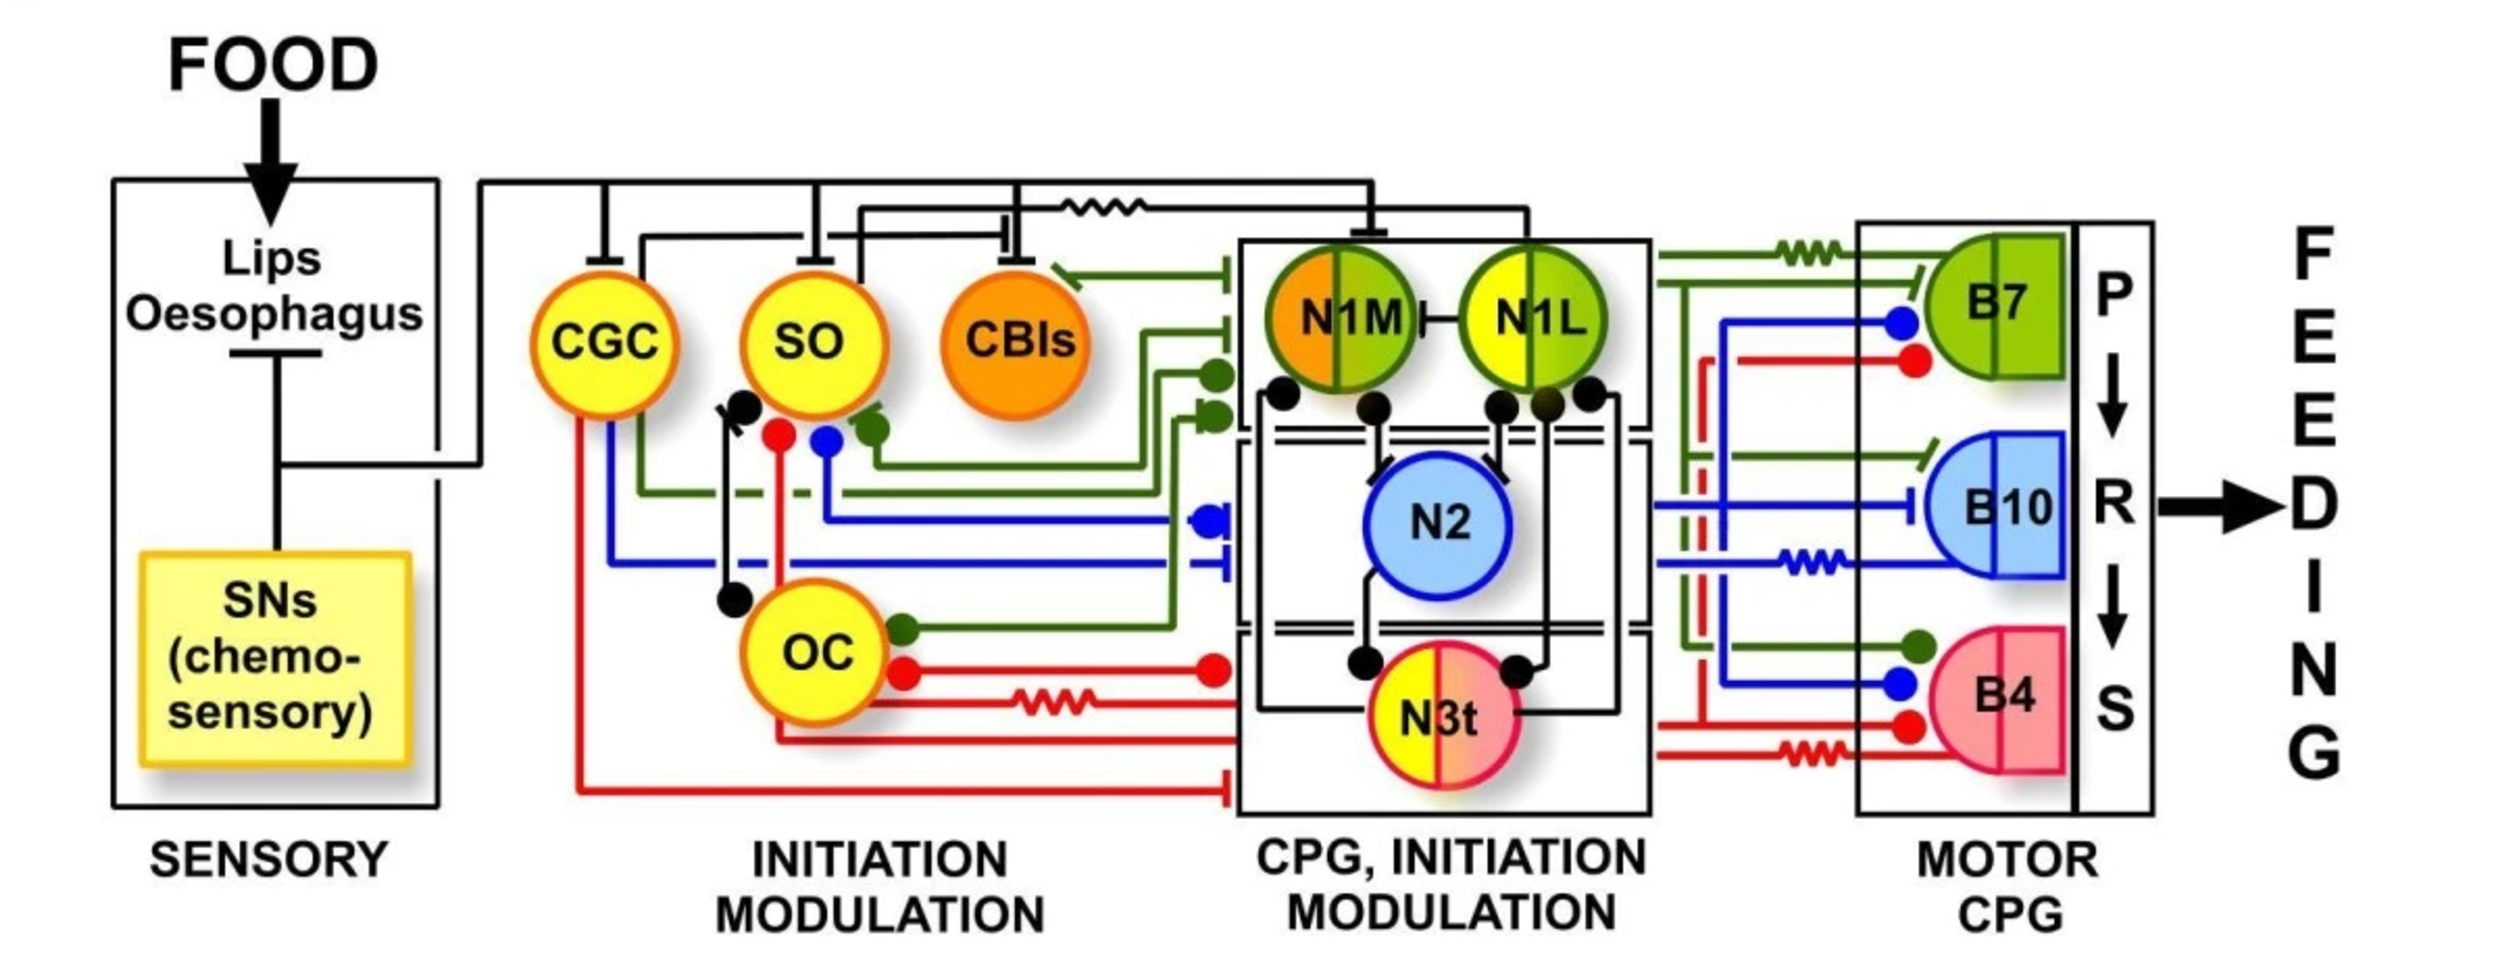
\includegraphics[width=\textwidth]{img/invariants/distributed_benjamin_2012.pdf}
	\caption{Representation of the distributed system of the feeding CPG. From left to right .... Dots indicate inhibitory chemical synapses, bars excitatory chemical synapses and resistor symbols electrotonic (electrical) synapses. Panel C from Figure 1 in \cite{benjamin_distributed_2012} (work under license \href{http://creativecommons.org/licenses/by/2.0}{Creative Commons Attribution})}
	%	Synaptic connectivity and functions of neurons in the feeding circuit. Modulatory function is indicated by yellow and initiating function by orange. CPG interneurons and motoneurons active during the three phases of the feeding rhythm are indicated by green (P = protraction), blue (R = rasp) and red (S = swallow). Neurons labeled with two colors have two functions. Dots indicate inhibitory chemical synapses, bars excitatory chemical synapses and resistor symbols electrotonic (electrical) synapses. This figure emphasizes the point that many of the neurons have more than function in the feeding network. See Abbreviations for all definitions of neuron types.
	\label{fig:feeding distribution}
\end{figure}






\subsubsection{Invariants in spontaneous activity}

\begin{figure}[htbp]
	\centering
	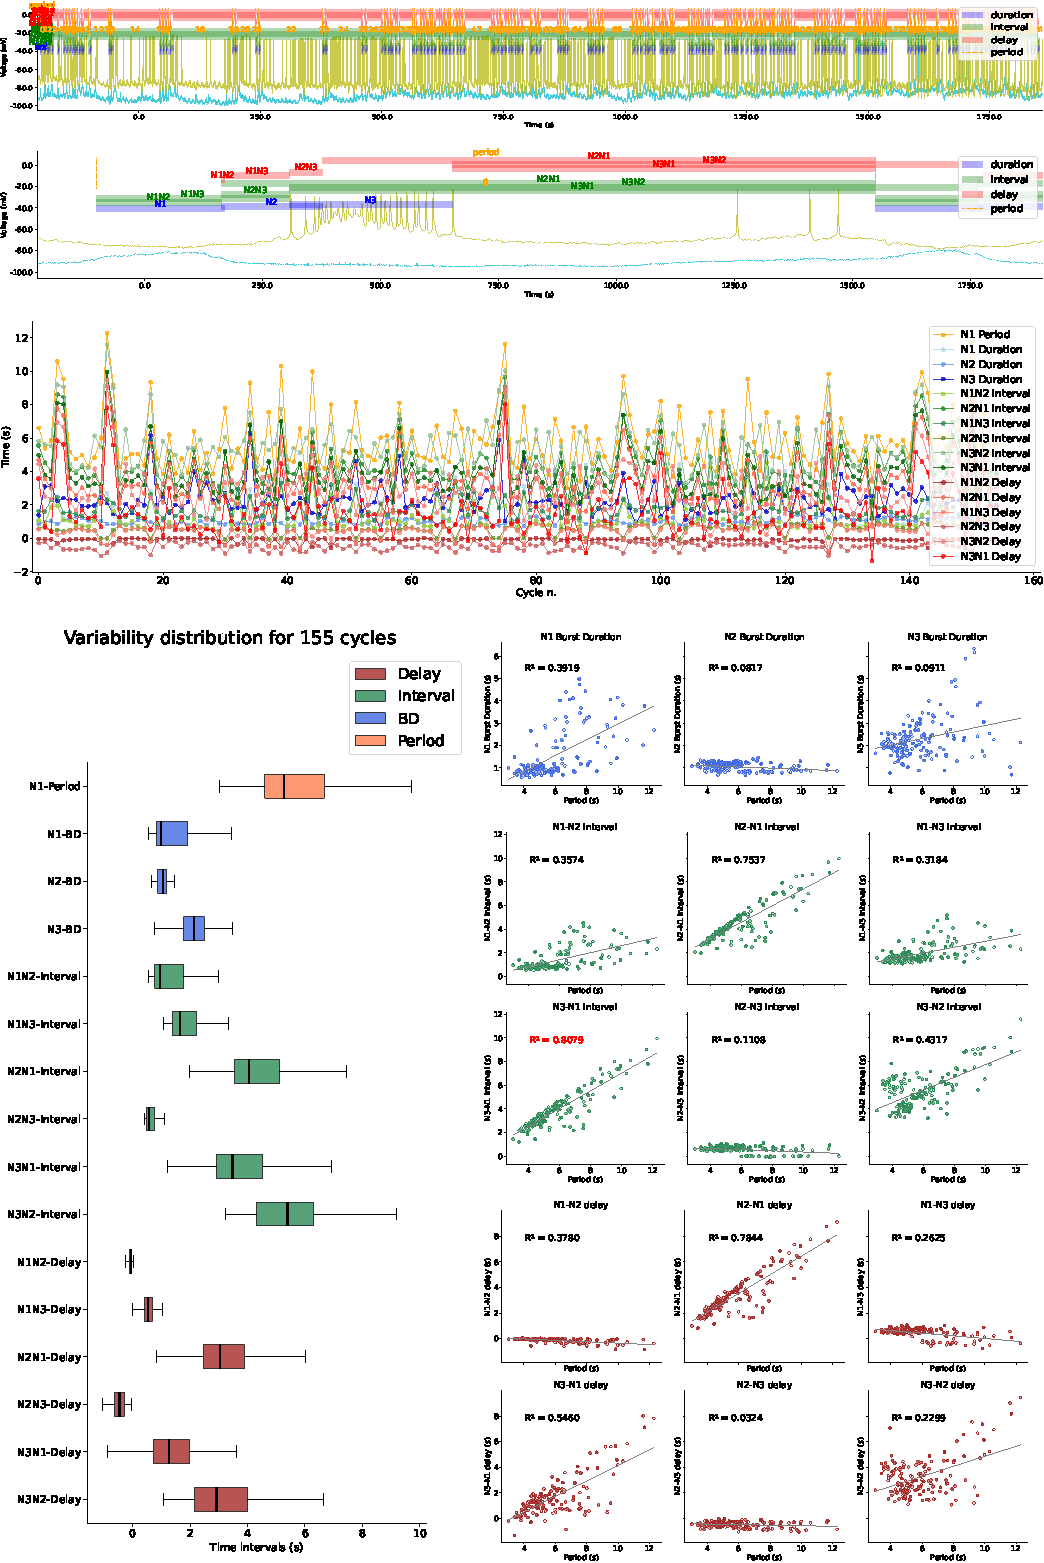
\includegraphics[width=1.1\textwidth]{./invariants/data/SUSSEX/prep1/images/3phases/panel_with_intervals.pdf}
	\caption{\textbf{Spontaneous case1}: Panel of intervals distribution and dynamical invariants for the three phases in the CPG for spontaneous activity.}
	\label{fig:prep1 invariants}
\end{figure}


\begin{figure}[htbp]
	\centering
	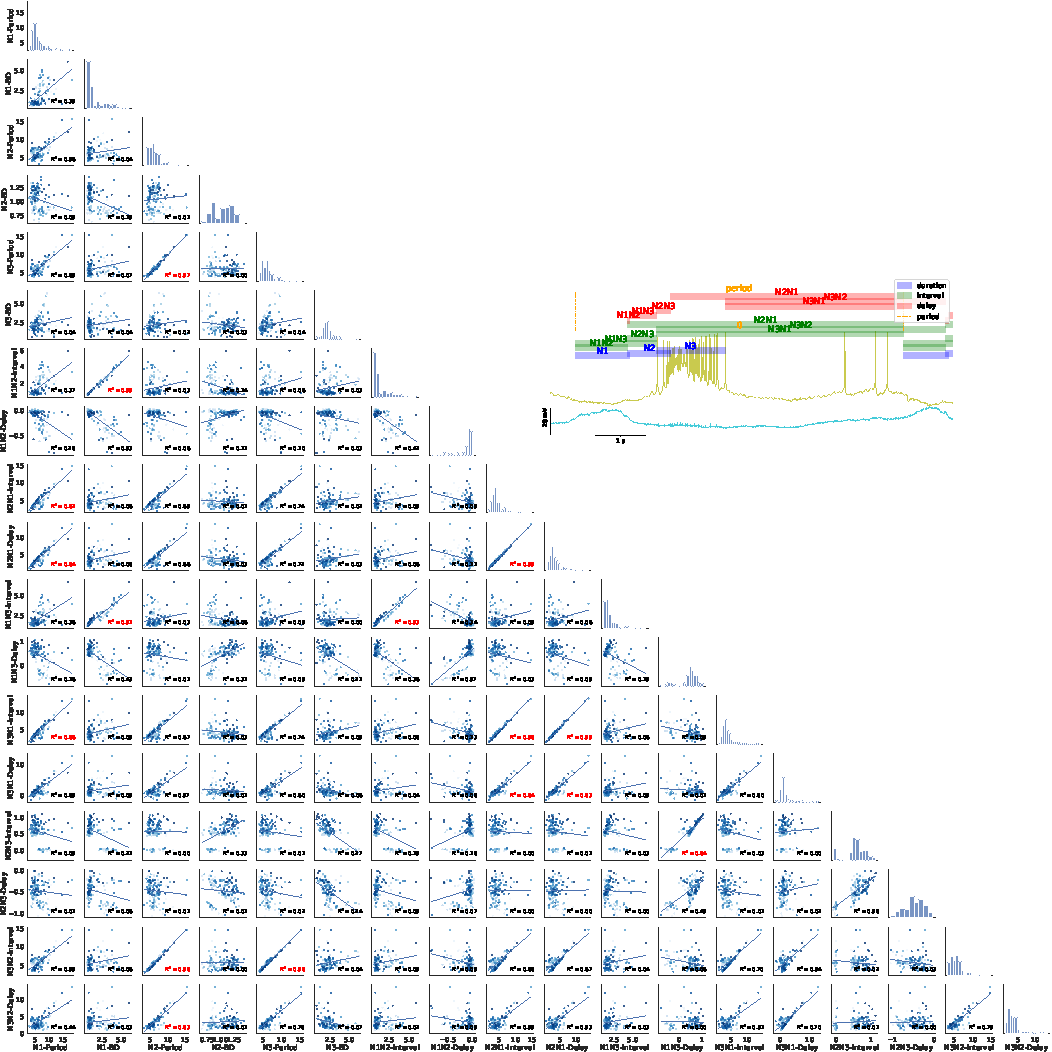
\includegraphics[width=1.1\textwidth]{./invariants/data/SUSSEX/prep1/images/3phases/panel_with_pairplot.pdf}
	\caption{\textbf{Spontaneous case1}: Panel of intervals distribution and dynamical invariants for the three phases in the CPG for spontaneous activity.}
	\label{fig:prep1 invariants pairplot}
\end{figure}


\begin{figure}[htbp]
	\centering
	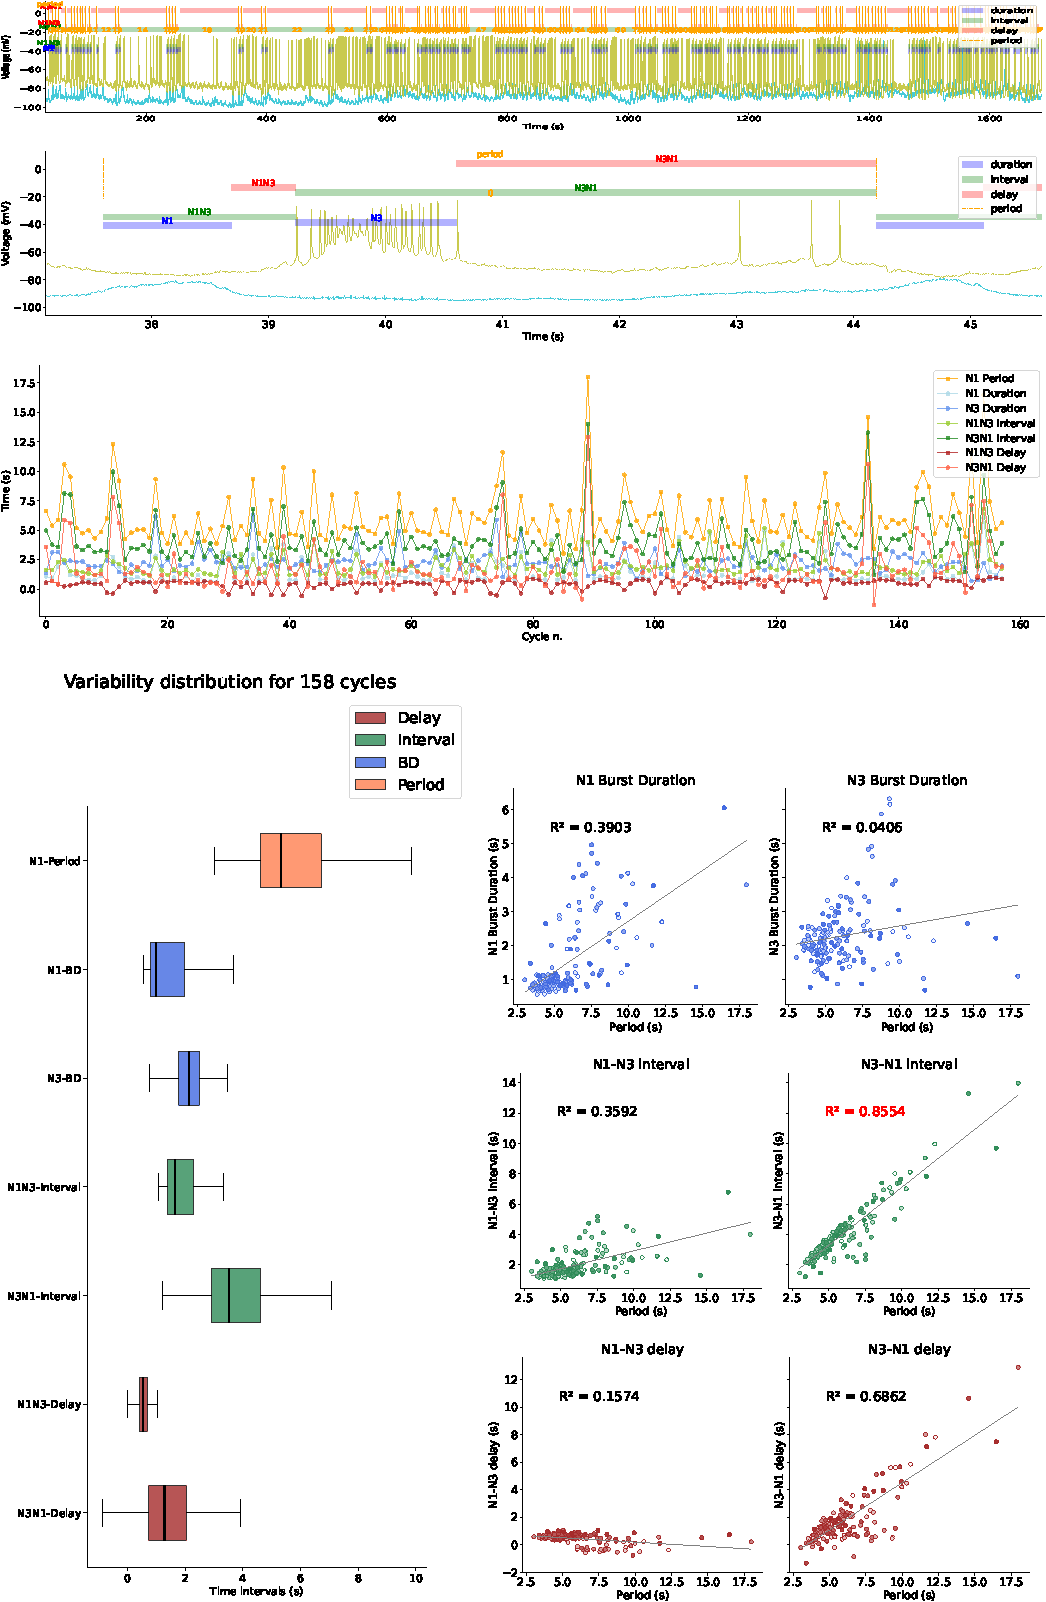
\includegraphics[width=1.1\textwidth]{./invariants/data/SUSSEX/prep1/images/2phases/panel_with_intervals.pdf}
	\caption{\textbf{Spontaneous case1}: Panel of intervals distribution and dynamical invariants for two phases in the CPG for spontaneous activity.}
	\label{fig:prep1 2 phases invariants}
\end{figure}
%
\begin{figure}[htbp]
	\centering
	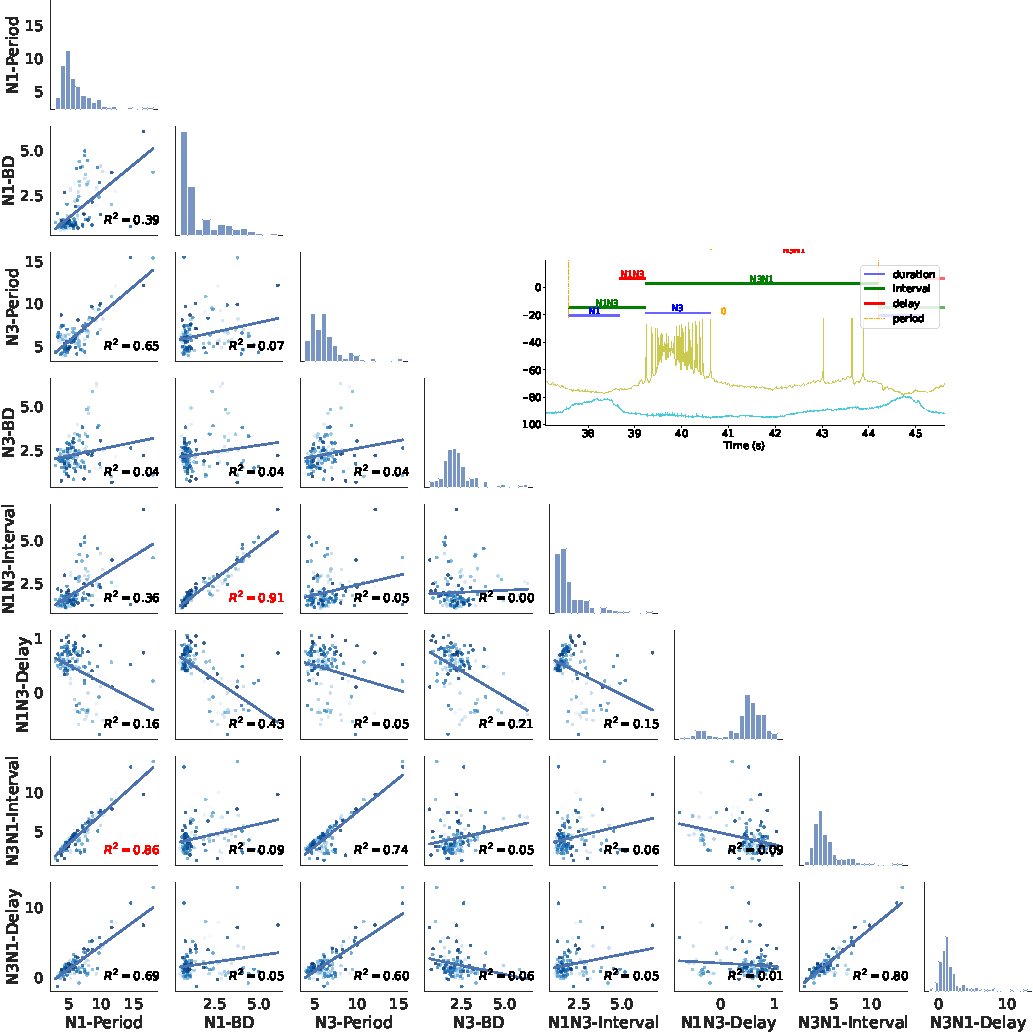
\includegraphics[width=1.1\textwidth]{./invariants/data/SUSSEX/prep1/images/2phases/panel_with_pairplot.pdf}
	\caption{\textbf{Spontaneous case1}: Panel of intervals distribution and dynamical invariants for the two phases in the CPG for spontaneous activity.}
	\label{fig:prep1 2 phases invariants pairplot}
\end{figure}


\begin{figure}[htbp]
	\centering
	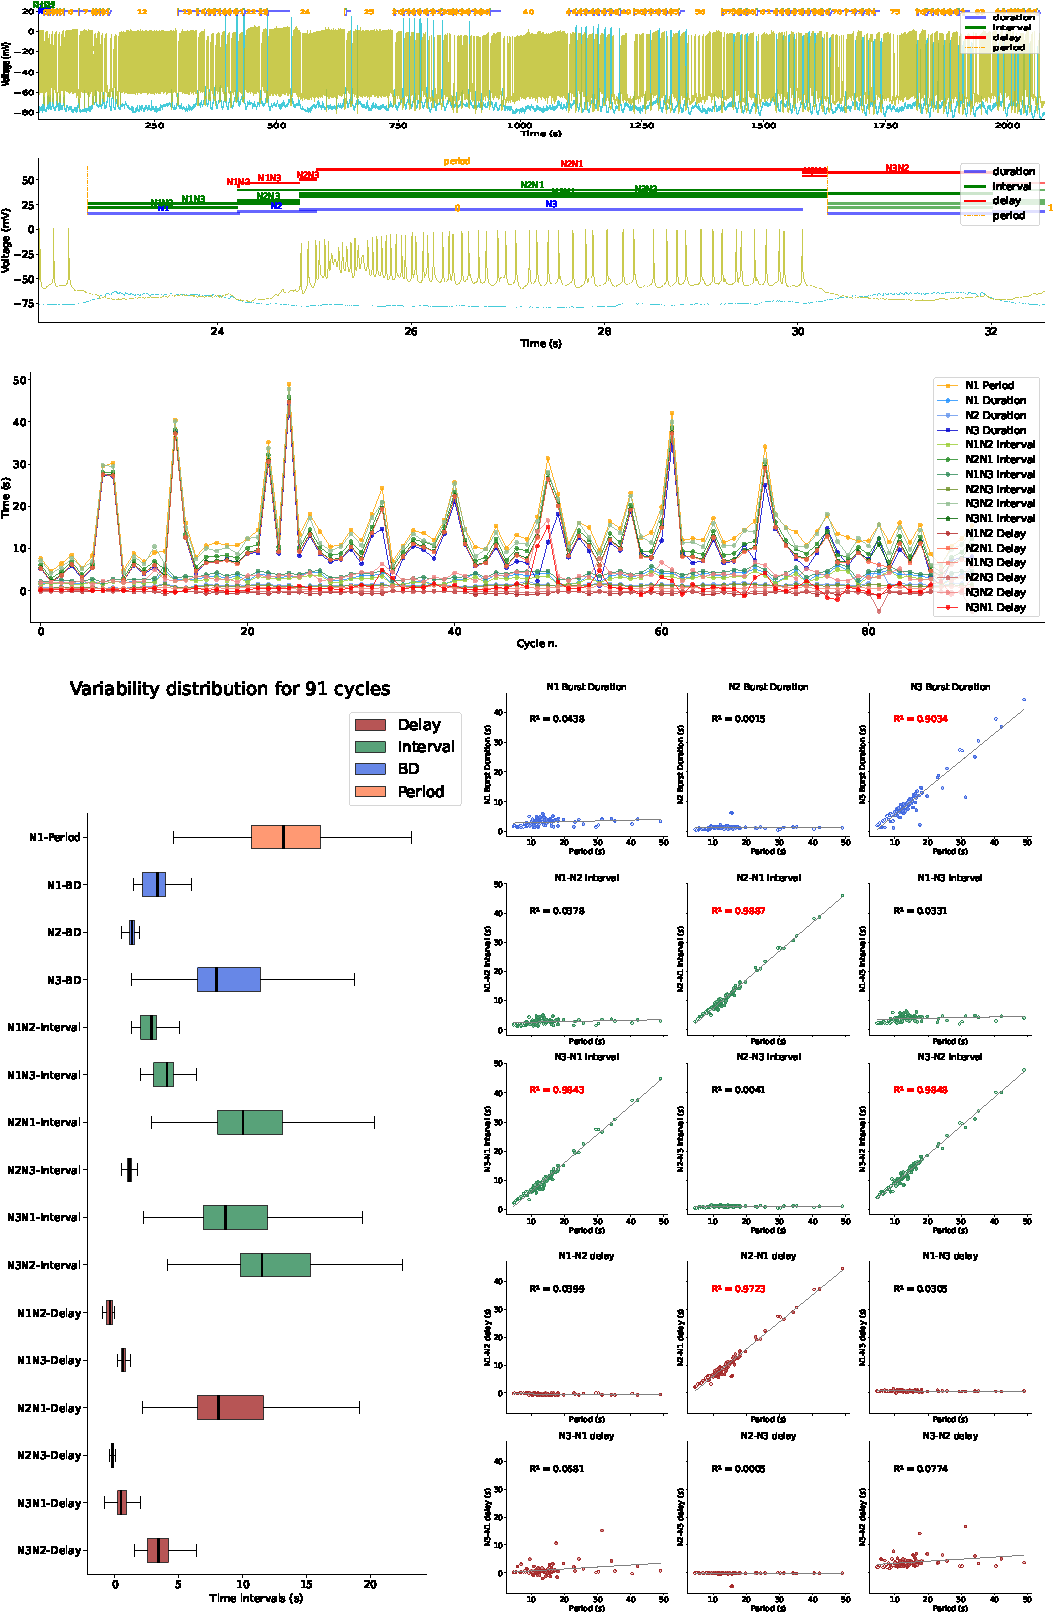
\includegraphics[width=1.1\textwidth]{./invariants/data/SUSSEX/prep2/images/3phases/panel_with_intervals.pdf}
	\caption{\textbf{Spontaneous case2}: Panel of intervals distribution and dynamical invariants for the three phases in the CPG for spontaneous activity.}
	\label{fig:prep2 invariants}
\end{figure}

\begin{figure}[htbp]
	\centering
	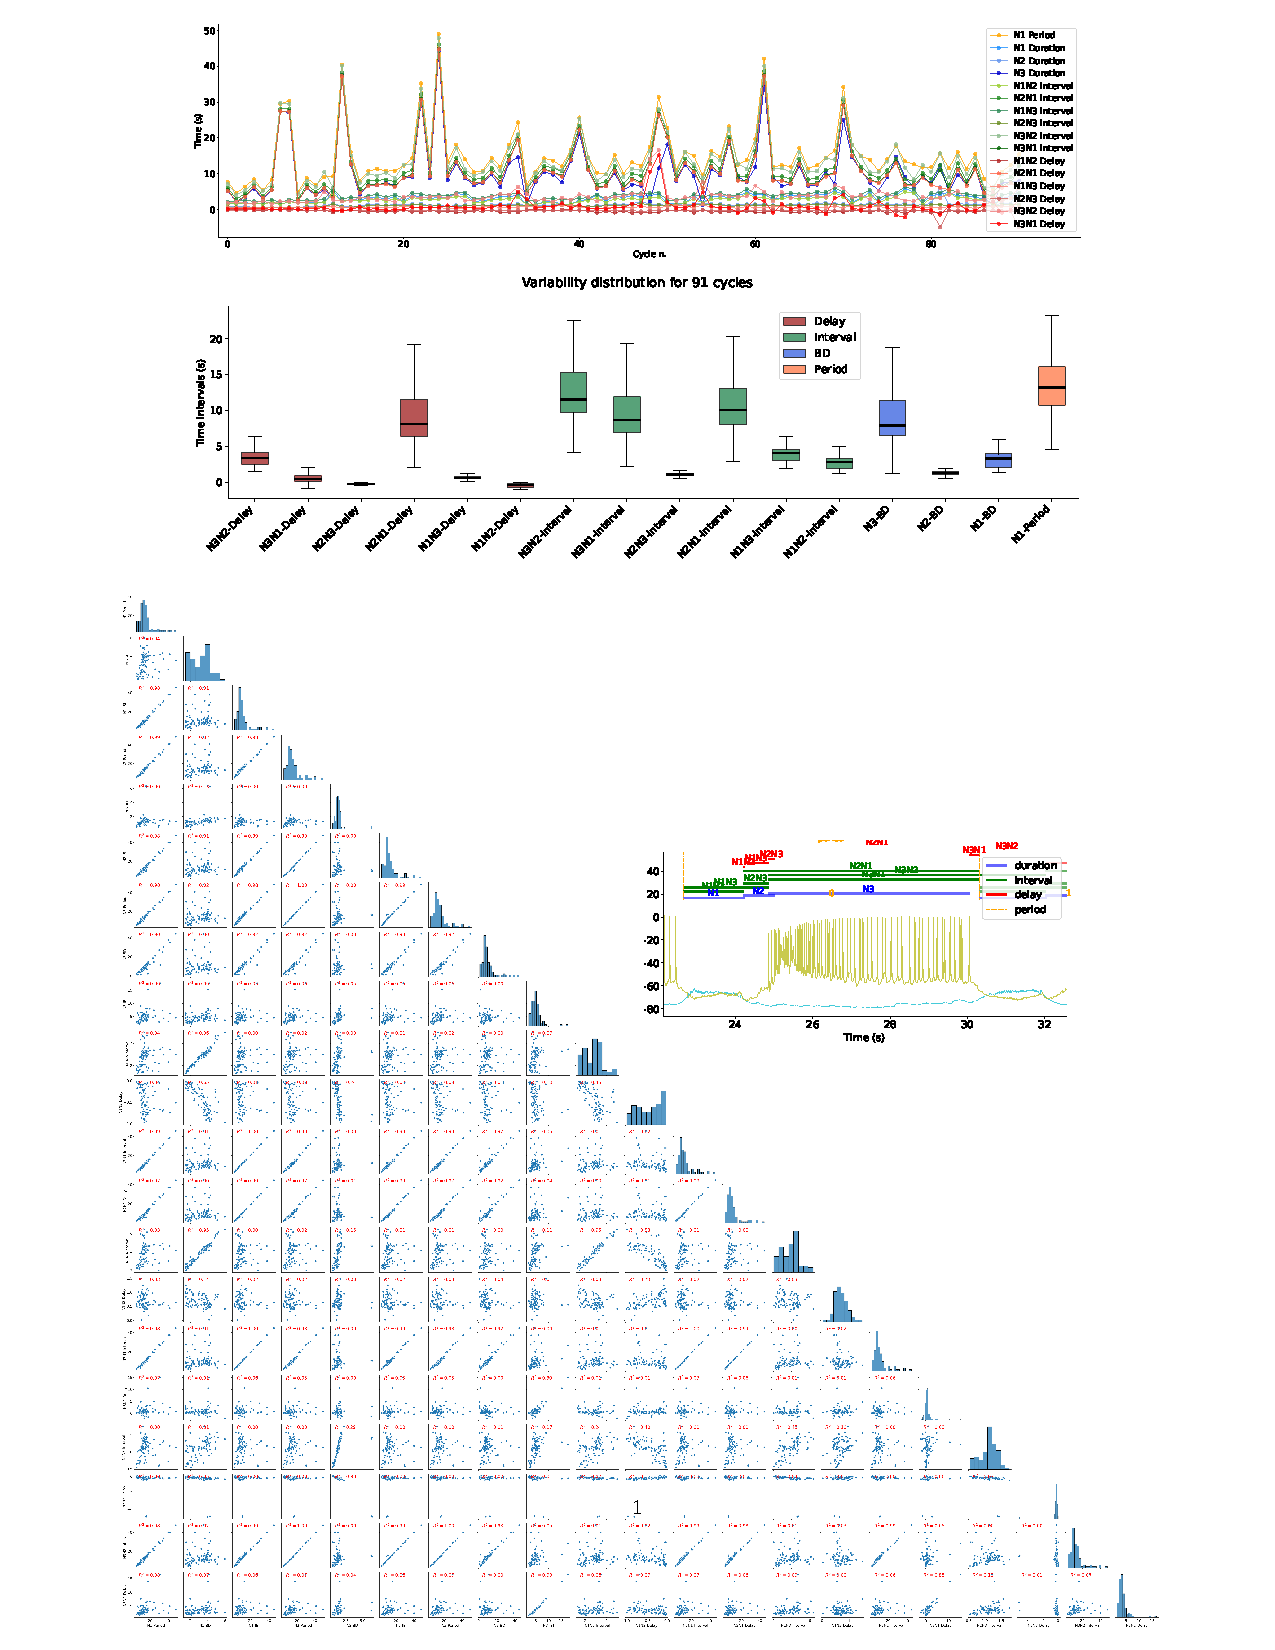
\includegraphics[width=1.1\textwidth]{./invariants/data/SUSSEX/prep2/images/3phases/panel_with_pairplot.pdf}
	\caption{\textbf{Spontaneous case2}: Panel of intervals distribution and dynamical invariants for the three phases in the CPG for spontaneous activity.}
	\label{fig:prep2 pairplot invariants}
\end{figure}


\begin{figure}[htbp]
	\centering
	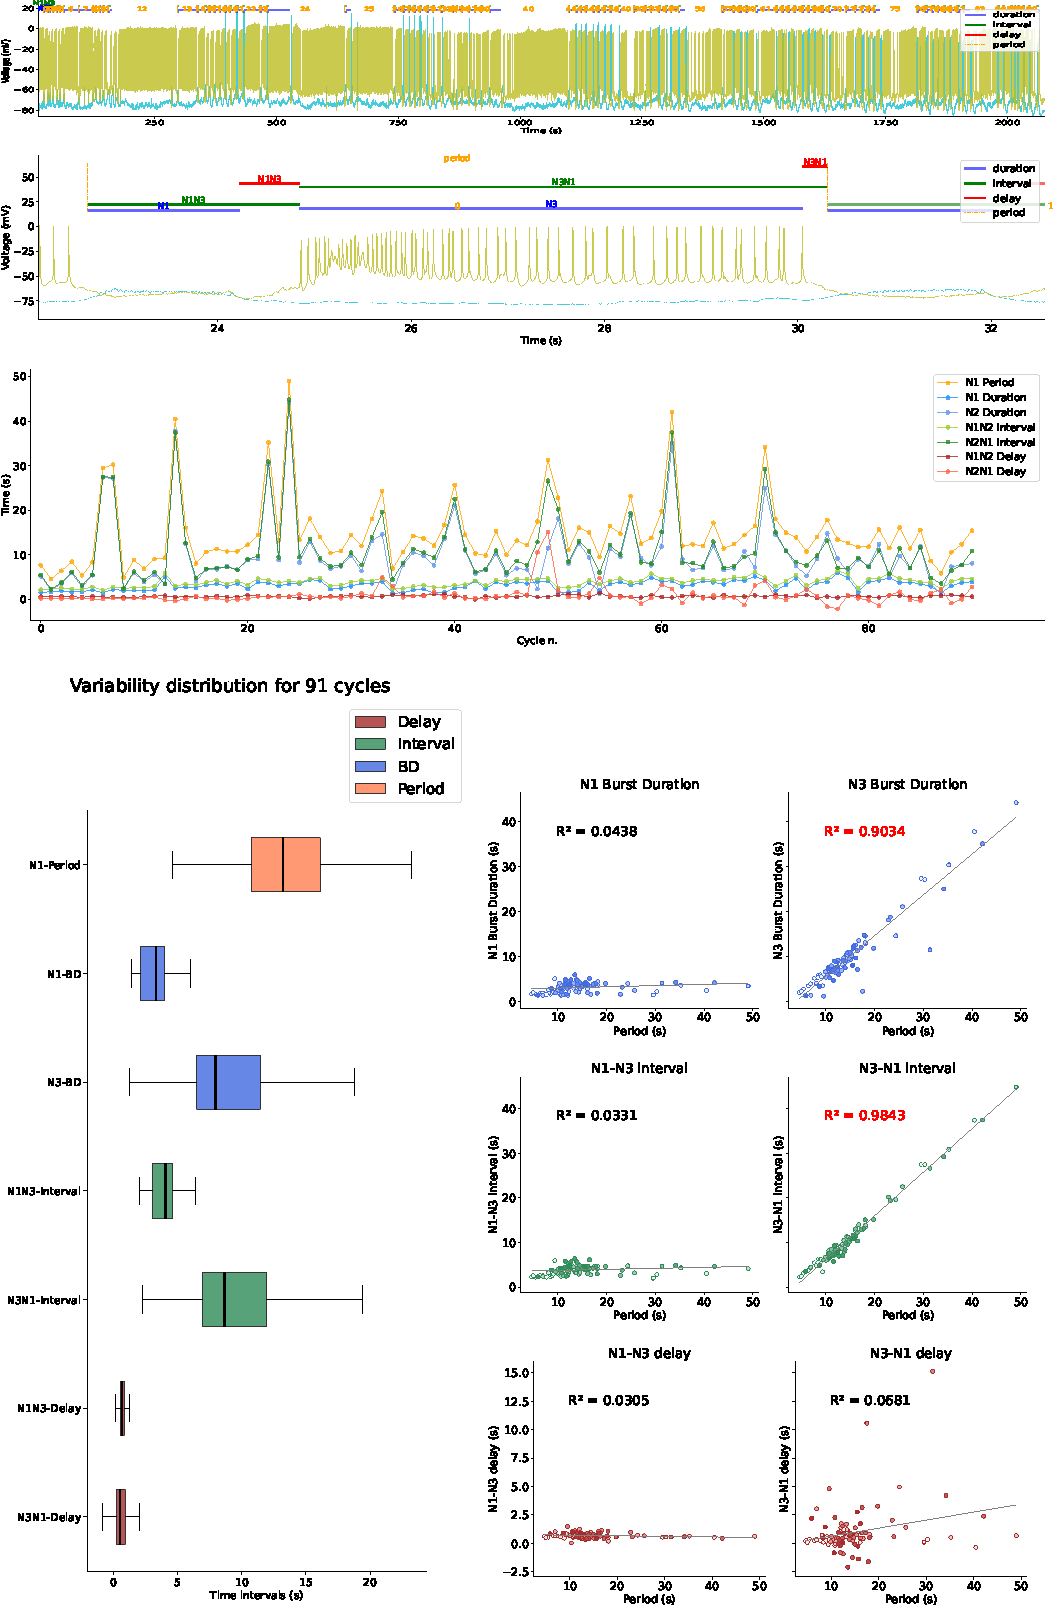
\includegraphics[width=1.1\textwidth]{./invariants/data/SUSSEX/prep2/images/2phases/panel_with_intervals.pdf}
	\caption{\textbf{Spontaneous case2}: Panel of intervals distribution and dynamical invariants for two phases in the CPG for spontaneous activity.}
	\label{fig:prep2 2phase invariants}
\end{figure}

\begin{figure}[htbp]
\centering
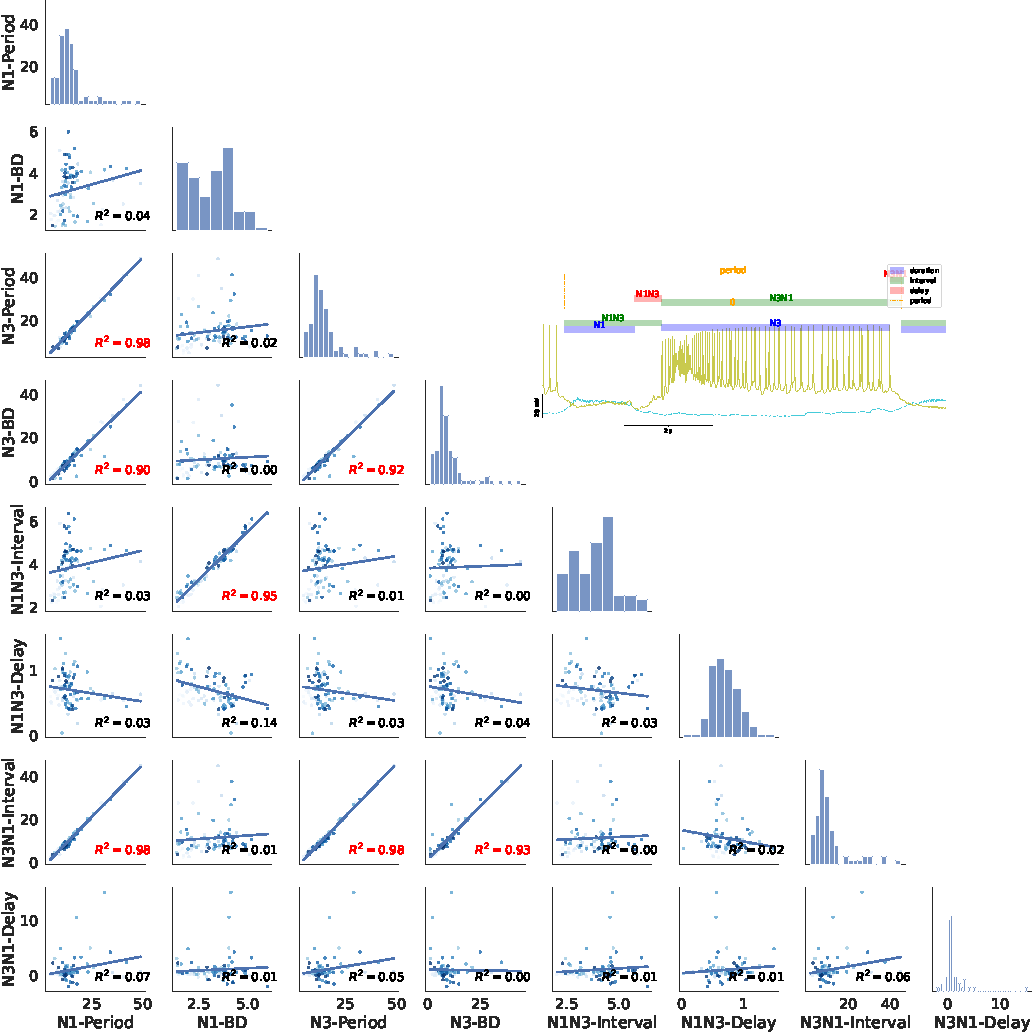
\includegraphics[width=1.1\textwidth]{./invariants/data/SUSSEX/prep2/images/2phases/panel_with_pairplot.pdf}
\caption{\textbf{Spontaneous case2}: Panel of intervals distribution and dynamical invariants for two phases in the CPG for spontaneous activity.}
\label{fig:prep2 2phase invariants pairplot}
\end{figure}


\begin{figure}[htbp]
	\centering
	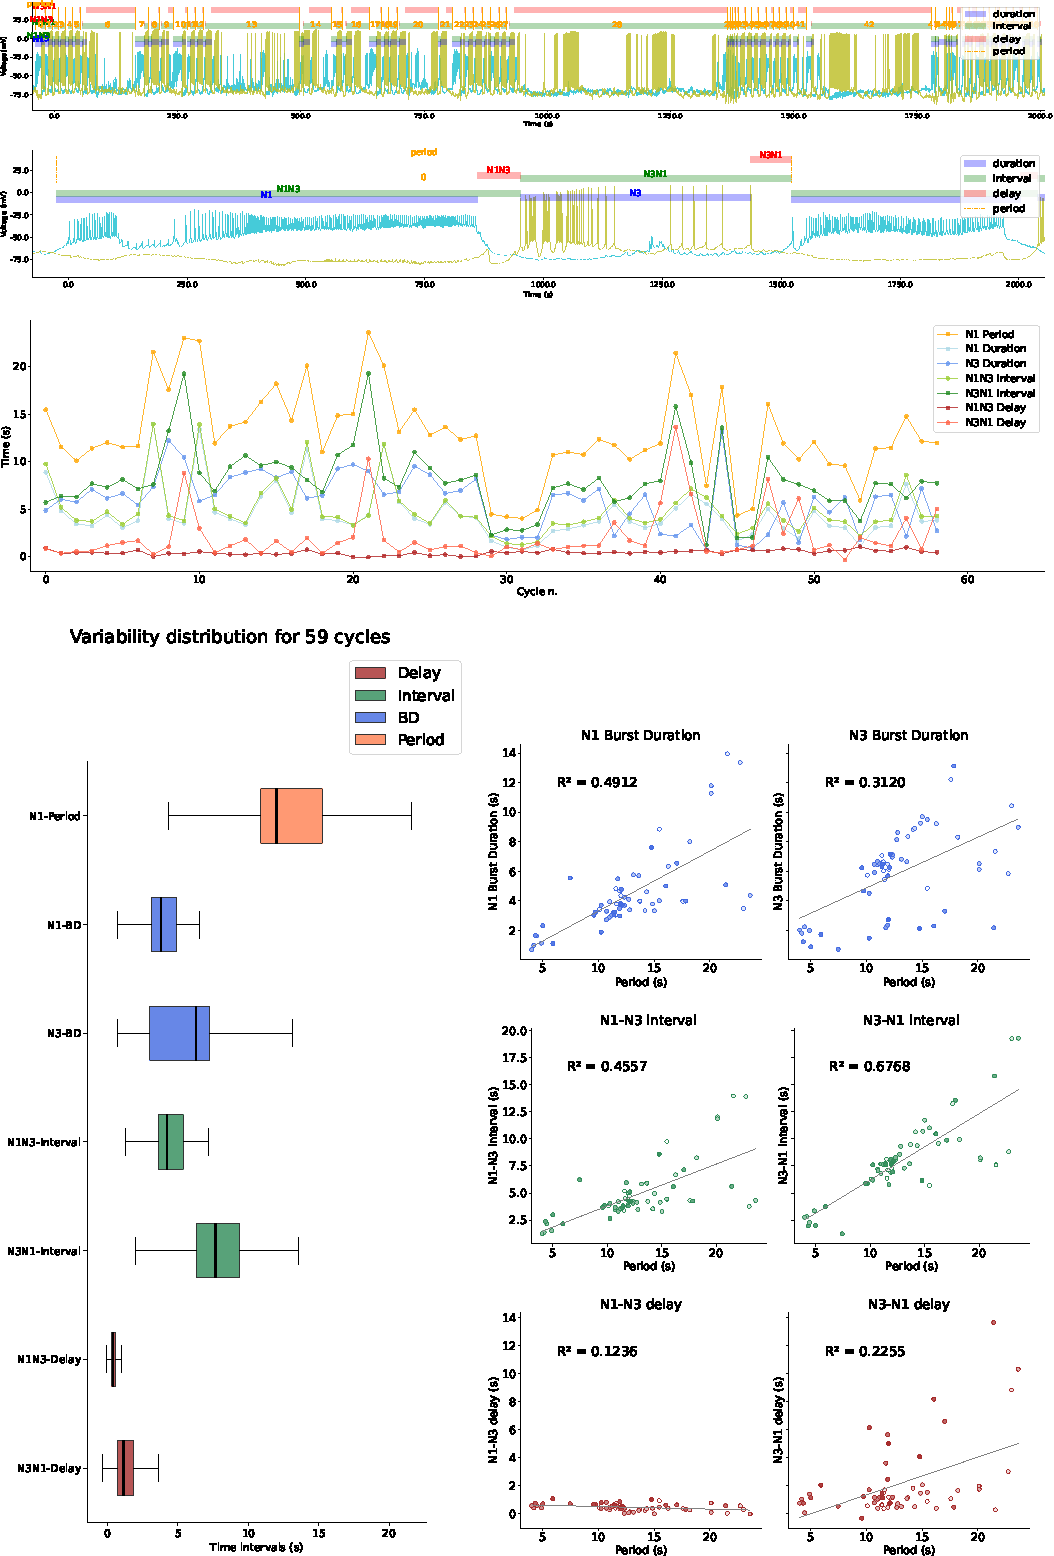
\includegraphics[width=1.1\textwidth]{./invariants/data/SUSSEX/prep3/images/2phases/panel_with_intervals.pdf}
	\caption{\textbf{Spontaneous case3}: Panel of intervals distribution and dynamical invariants for two phases in the CPG for spontaneous activity.}
	\label{fig:prep3 2phases invariants}
\end{figure}

\begin{figure}[htbp]
\centering
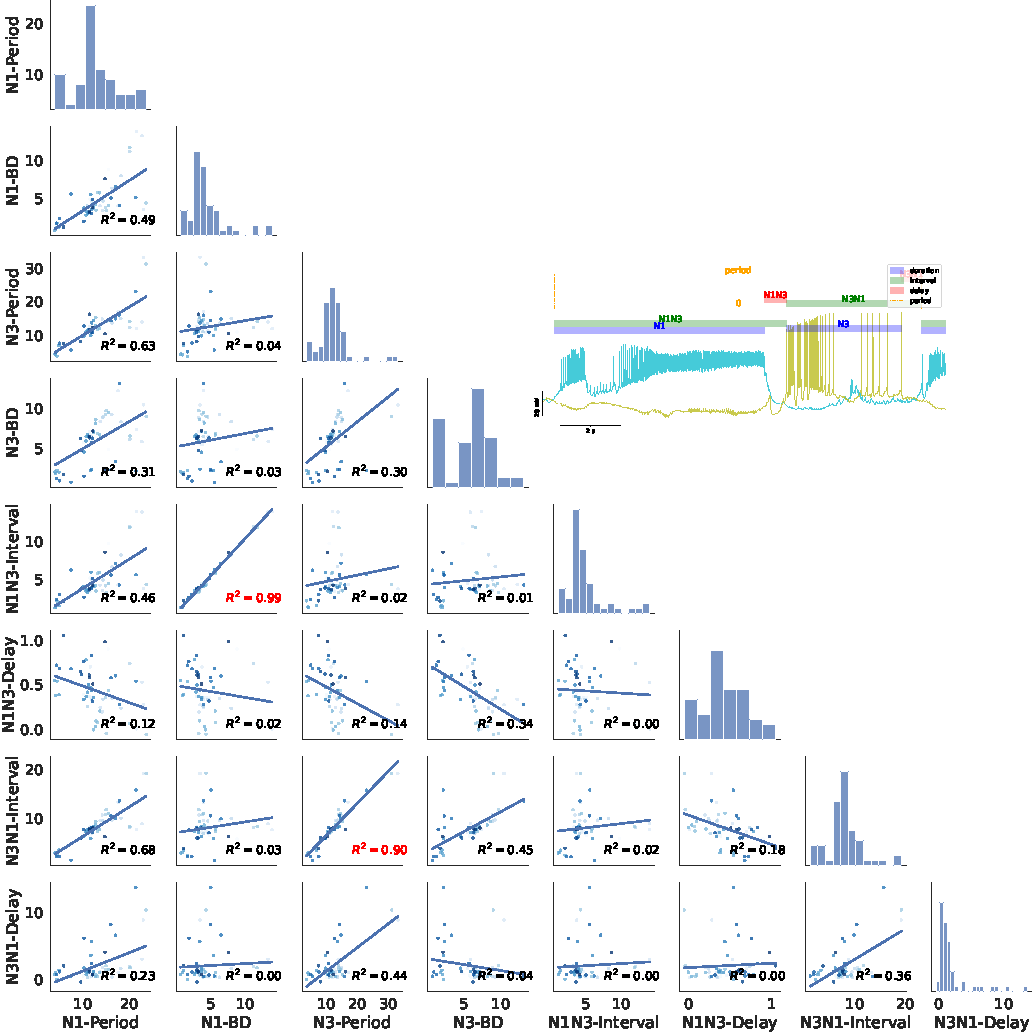
\includegraphics[width=1.1\textwidth]{./invariants/data/SUSSEX/prep3/images/2phases/panel_with_pairplot.pdf}
\caption{\textbf{Spontaneous case3}: Panel of intervals distribution and dynamical invariants for two phases in the CPG for spontaneous activity.}
\label{fig:prep3 2phases invariants pairplot}
\end{figure}

\begin{figure}[htbp]
	\centering
	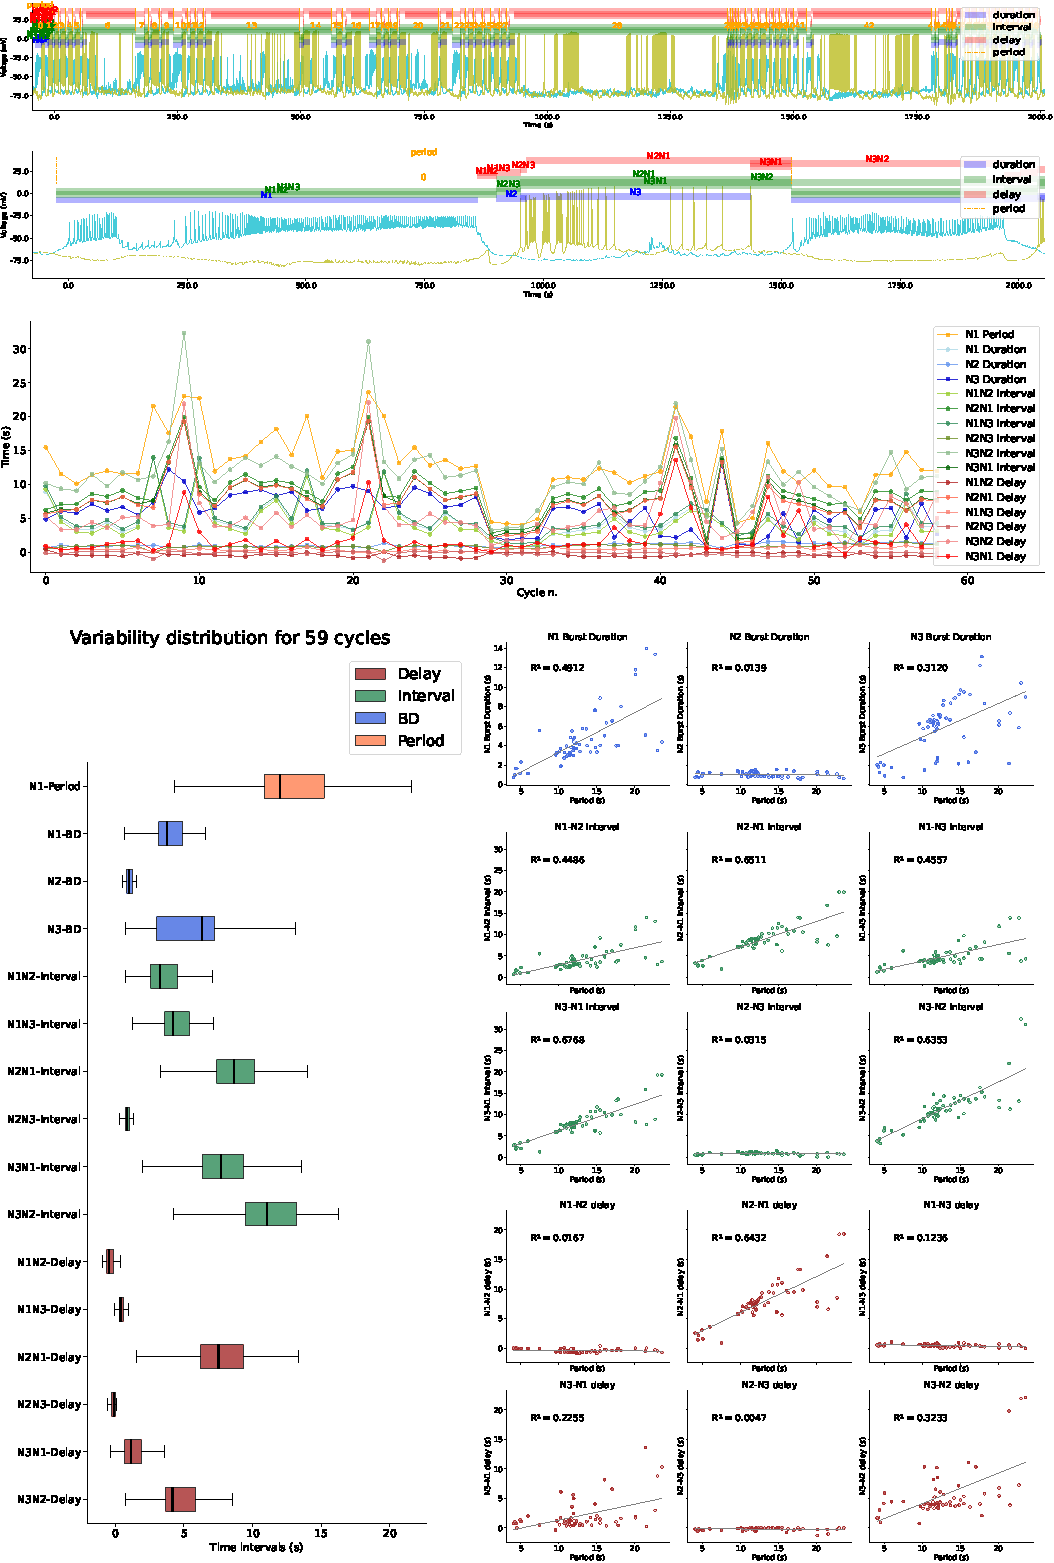
\includegraphics[width=1.1\textwidth]{./invariants/data/SUSSEX/prep3/images/3phases/panel_with_intervals.pdf}
	\caption{\textbf{Spontaneous case3}: Panel of intervals distribution and dynamical invariants for the three phases in the CPG for spontaneous activity.}
	\label{fig:prep3 invariants}
\end{figure}

\begin{figure}[htbp]
	\centering
	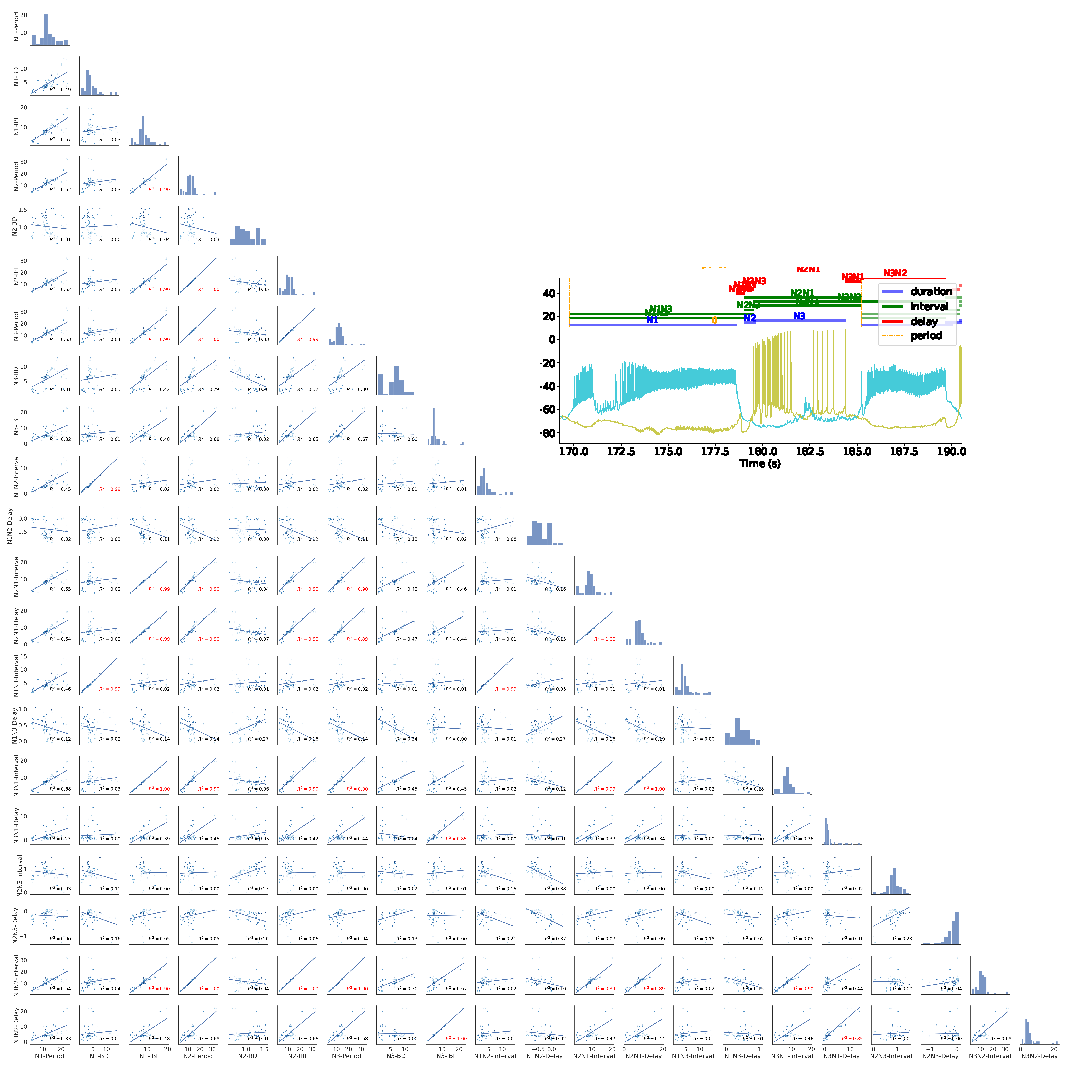
\includegraphics[width=1.1\textwidth]{./invariants/data/SUSSEX/prep3/images/3phases/panel_with_pairplot.pdf}
	\caption{\textbf{Spontaneous case3}: Panel of intervals distribution and dynamical invariants for the three phases in the CPG for spontaneous activity.}
	\label{fig:prep3 invariants pairplot}
\end{figure}


\subsubsection{Invariants in SO driven activity}
\paragraph{1. Spontaneous SO modulation recording}
% Nota: datos de preparación 4 en la detección está solo n1m y b8, las fases son N1 y N3. 
 
\begin{figure}[htbp]
	\centering
	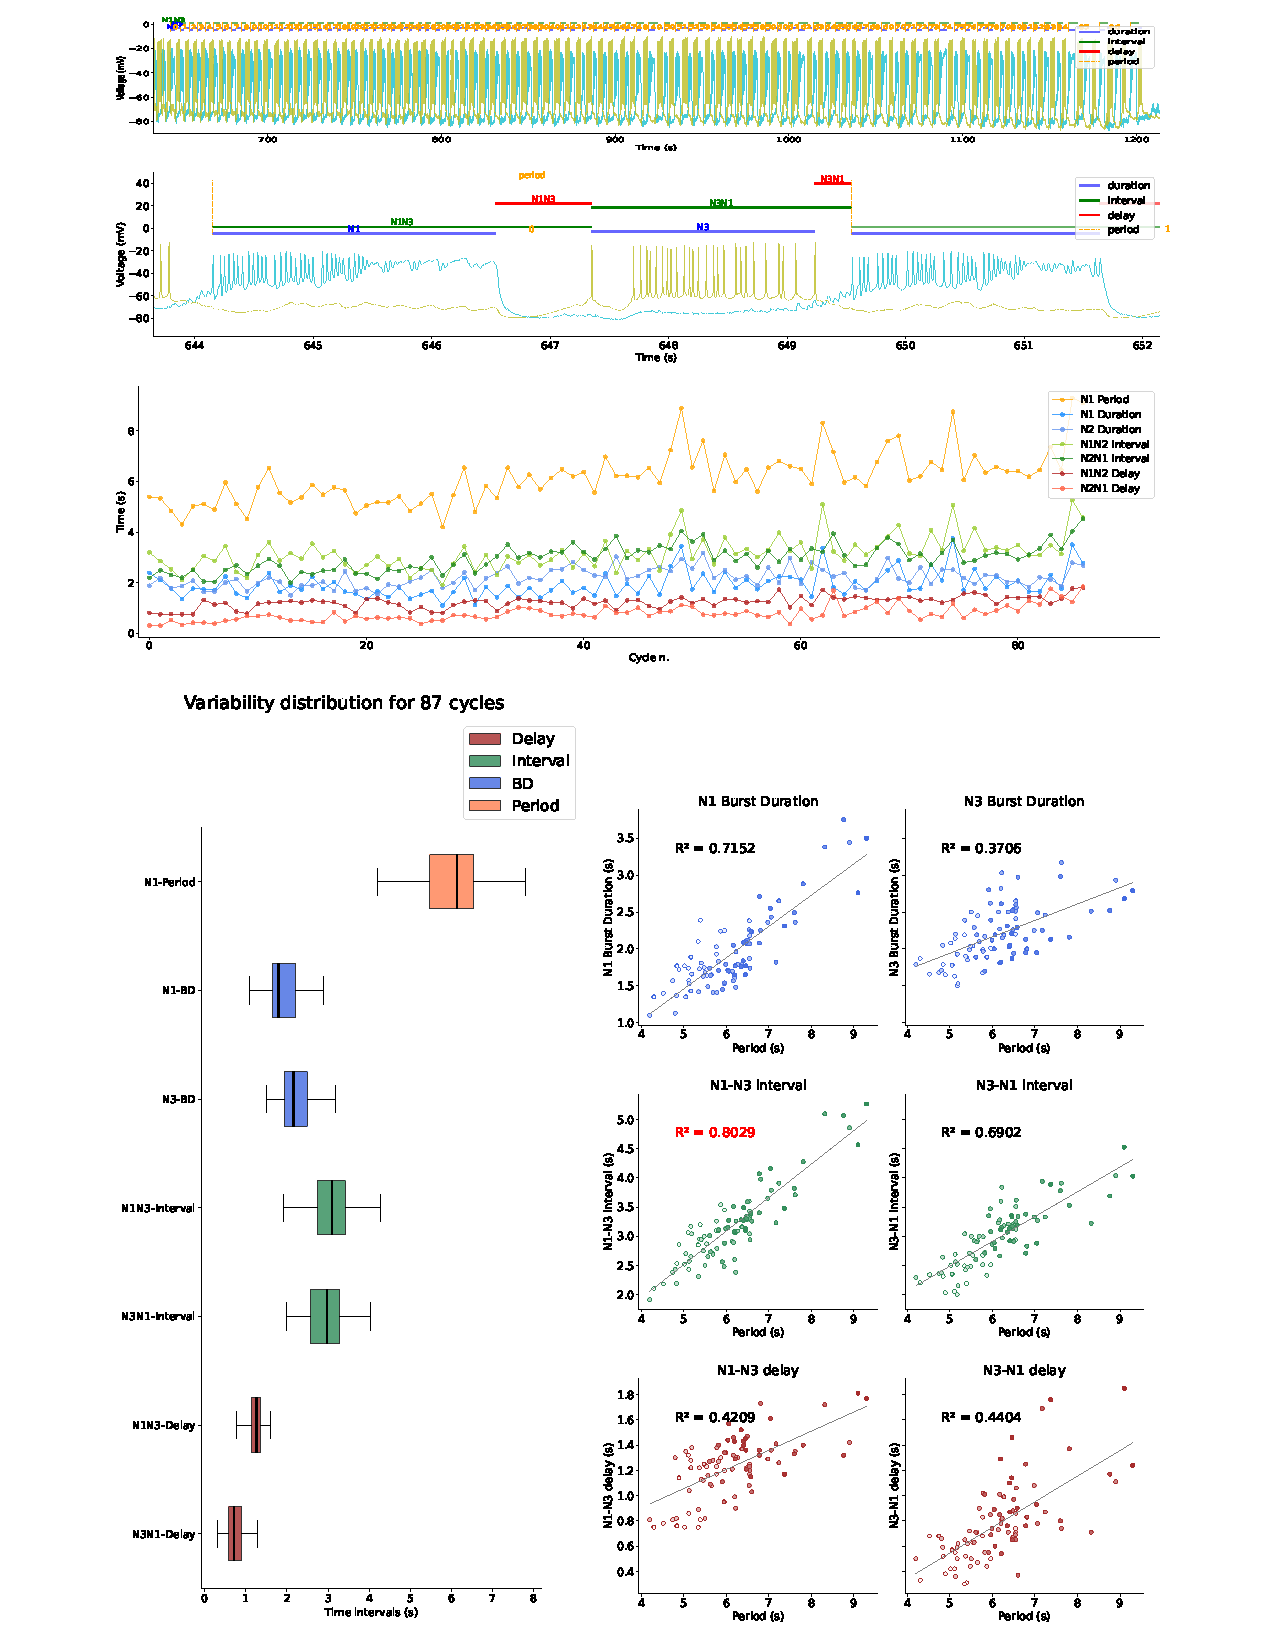
\includegraphics[width=1.1\textwidth]{./invariants/data/SUSSEX/prep4_so_driven_2/images/panel_with_intervals.pdf}
	\caption{\textbf{Spontaneous SO neuron driven}: Panel of intervals distribution and dynamical invariants for the three phases in the CPG for spontaneous activity driven by SO neuron.}
	\label{fig:so spontaneous invariants}
\end{figure}

\begin{figure}[htbp]
	\centering
	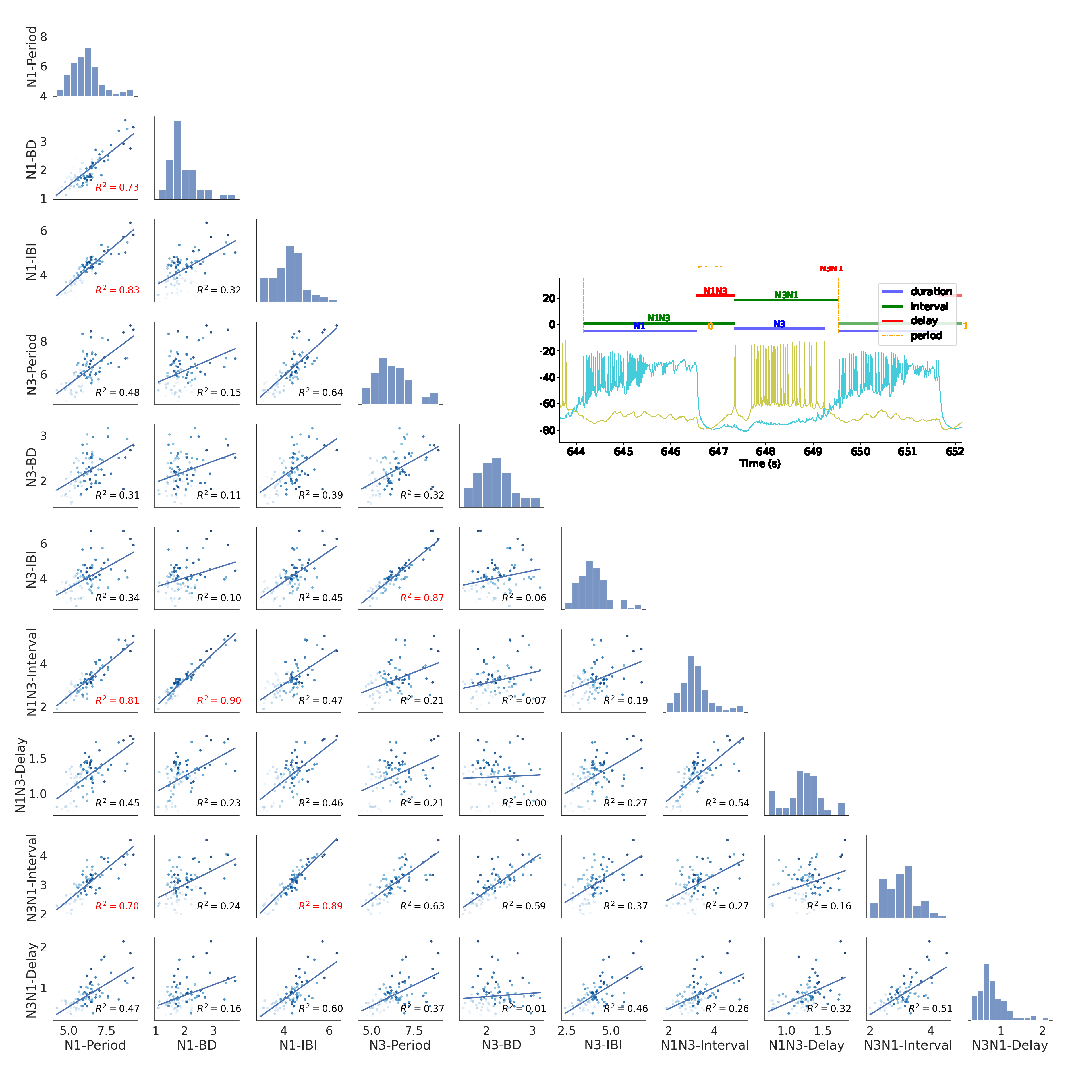
\includegraphics[width=1.1\textwidth]{./invariants/data/SUSSEX/prep4_so_driven_2/images/panel_with_pairplot.pdf}
	\caption{\textbf{Spontaneous SO neuron driven}: Panel of intervals distribution and dynamical invariants for the three phases in the CPG for spontaneous activity driven by SO neuron.}
	\label{fig:so spontaneous invariants pairplot}
\end{figure}
 	


\begin{figure}[htbp]
	\centering
	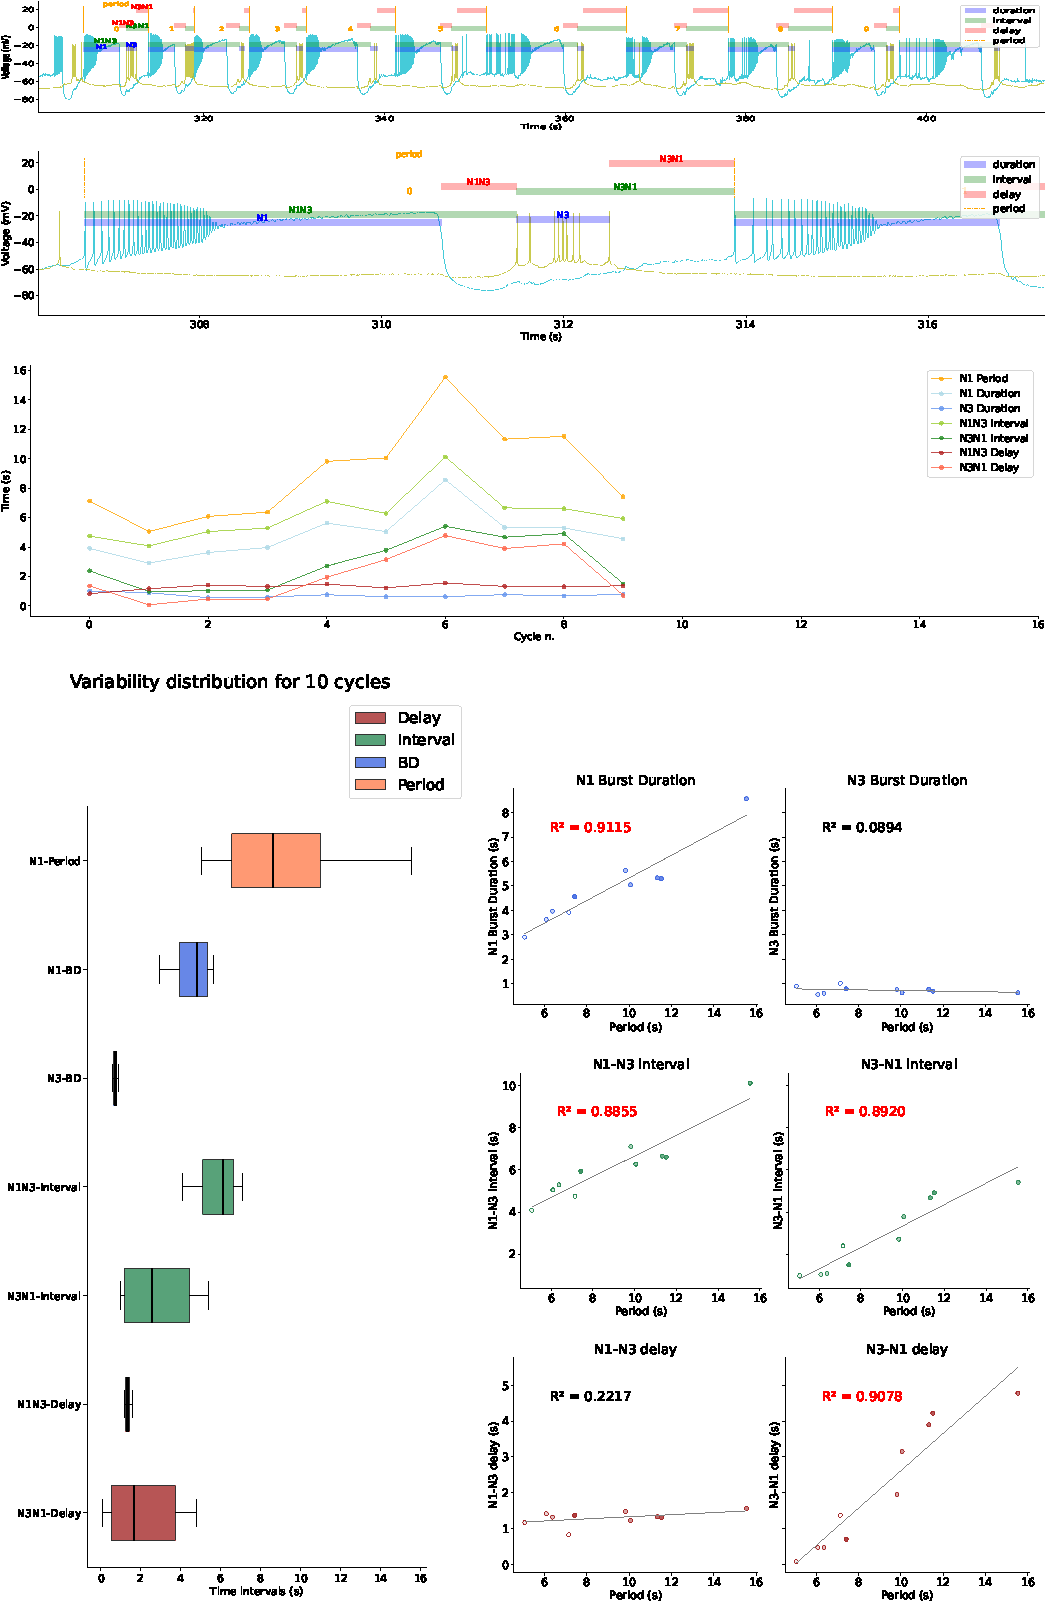
\includegraphics[width=1.1\textwidth]{./invariants/data/SUSSEX/prep4_so_no_driven/images/panel_with_intervals.pdf}
	\caption{\textbf{Spontaneous activity when SO-driven is over}: Panel of intervals distribution and dynamical invariants for the three phases in the CPG for spontaneous activity.}
	\label{fig:no so spontaneous invariants}
\end{figure}
 	 
 
\begin{figure}[htbp]
	\centering
	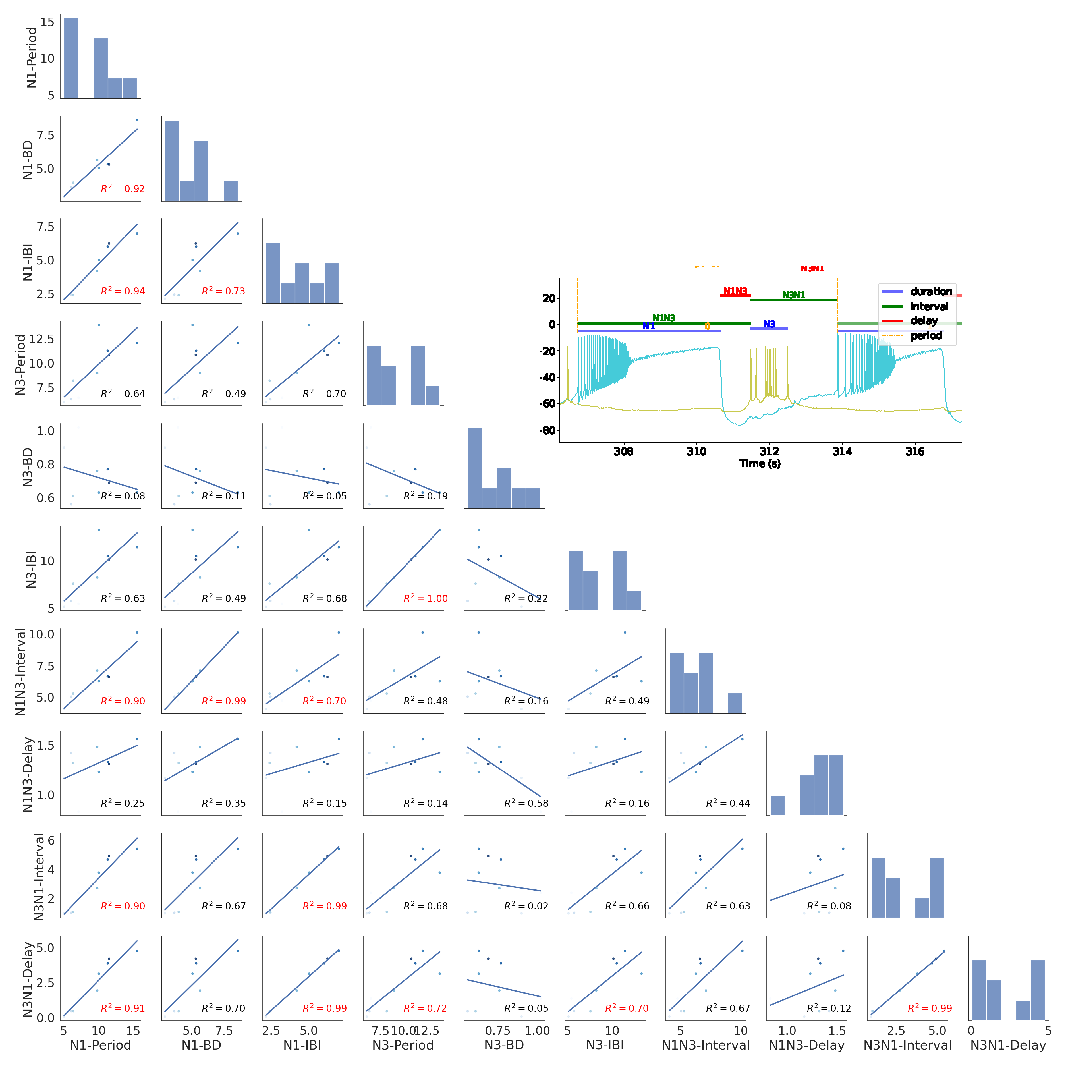
\includegraphics[width=1.1\textwidth]{./invariants/data/SUSSEX/prep4_so_no_driven/images/panel_with_pairplot.pdf}
	\caption{\textbf{Spontaneous activity when SO-driven is over}: Panel of intervals distribution and dynamical invariants for the three phases in the CPG for spontaneous activity.}
	\label{fig:no so spontaneous invariants pairplot}
\end{figure}
 
\paragraph{2. Stimulated SO recording}


\begin{figure}[htbp]
	\centering
	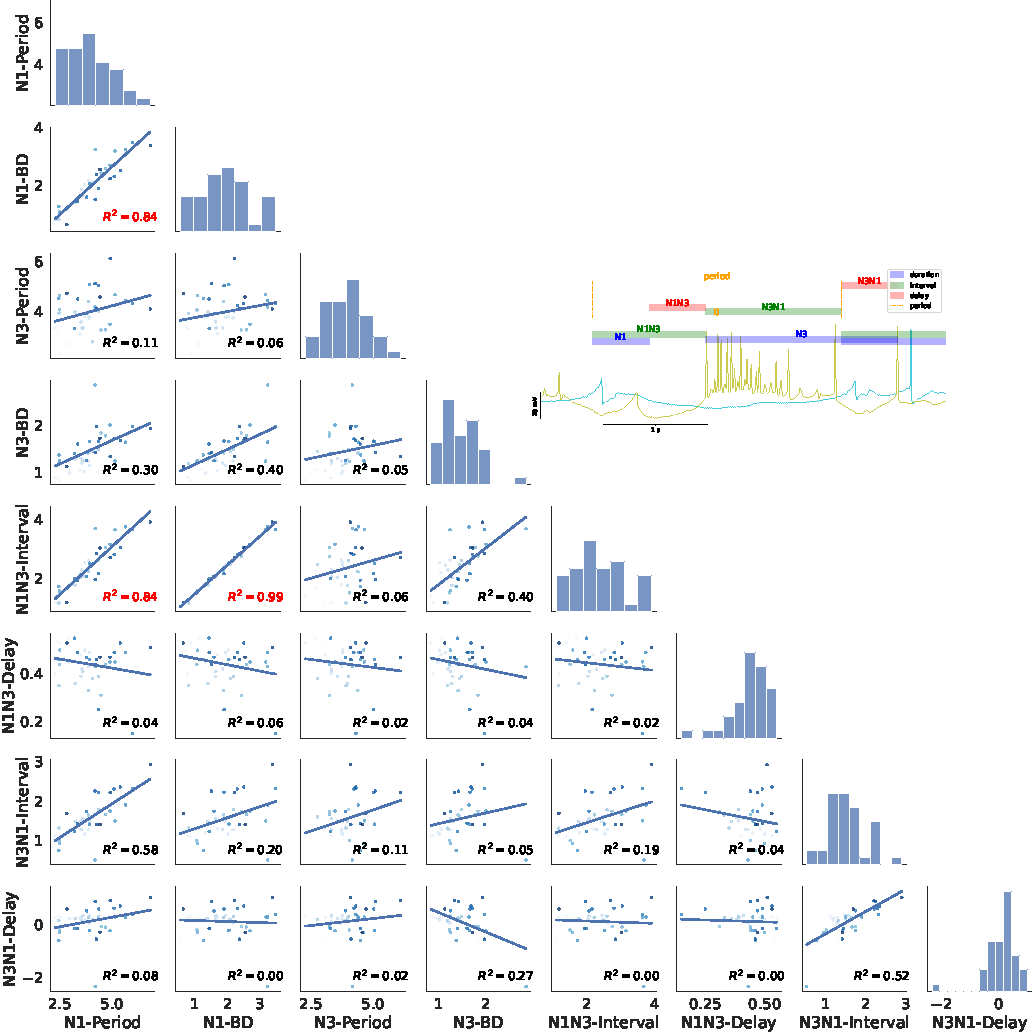
\includegraphics[width=1.1\textwidth]{./invariants/data/SUSSEX/SO_driven/images/panel_with_pairplot.pdf}
	\caption{\textbf{SO driven stimulation}: Panel of intervals distribution and dynamical invariants for the three phases in the CPG under SO modulatory neuron stimulation.}
	\label{fig:so stimulation pairplot}
\end{figure}



\subsubsection{Invariants in MLN stimulation driven activity}
The snail's lips are connected to the cerebral ganglia by the MLN (median lip nerves). It is possible to stimulate CPG activity by its stimulation, simulating the initiation of the rhythm in food presence \parencite{staras_electrophysiological_2019}. The data in this recording was stimulated by (4volt 1Hz stim).


\begin{figure}[htbp]
	\centering
	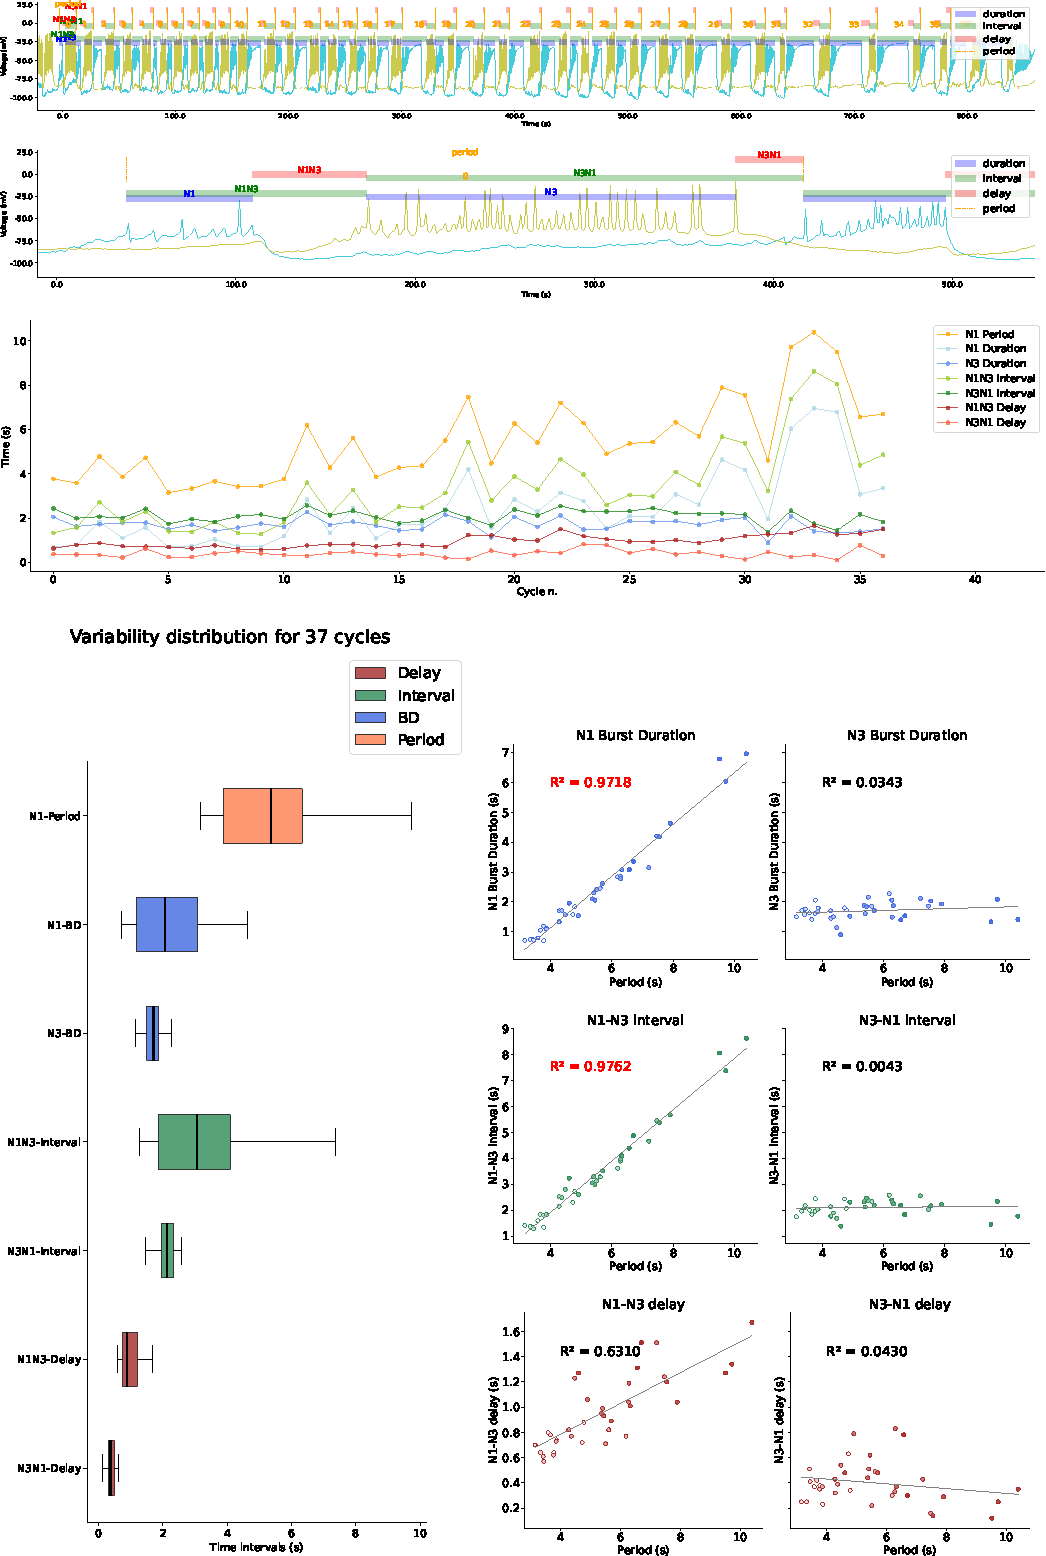
\includegraphics[width=1.1\textwidth]{./invariants/data/SUSSEX/MLN_driven/images/panel_with_intervals.pdf}
	\caption{\textbf{CV1a driven case 4}: Panel of intervals distribution and dynamical invariants for the three phases in the CPG under MLN Medium Lip Nerve (MLN) stimulation.}
	\label{fig:mln stimulation}
\end{figure}


\begin{figure}[htbp]
	\centering
	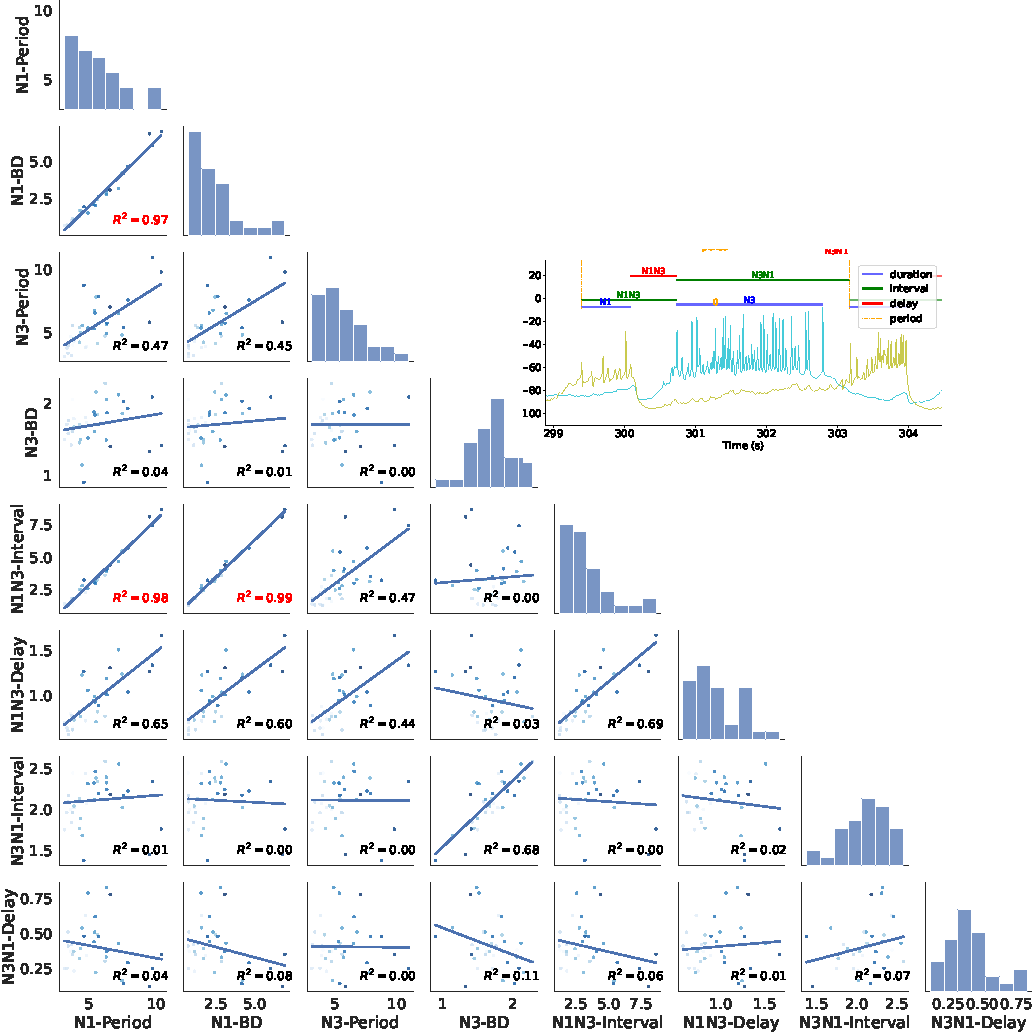
\includegraphics[width=1.1\textwidth]{./invariants/data/SUSSEX/MLN_driven/images/panel_with_pairplot.pdf}
	\caption{\textbf{CV1a driven case 4}: Panel of intervals distribution and dynamical invariants for the three phases in the CPG under MLN Medium Lip Nerve (MLN) stimulation.}
	\label{fig:mln stimulation pairplot}
\end{figure}

\subsubsection{Invariants in cva1 stimulation driven activity}
CV1a is part of a larger population of CBIs 
%and the complete map of their locations is shown in Figure 3A. https://static-content.springer.com/esm/art%3A10.1186%2F2042-1001-2-4/MediaObjects/13232_2011_20_MOESM3_ESM.jpeg
Sucrose drives rhythmic activity in CBIs activating the feeding circuit by the conection
\paragraph{\large{Example 1}}

\begin{figure}[htbp]
	\centering
	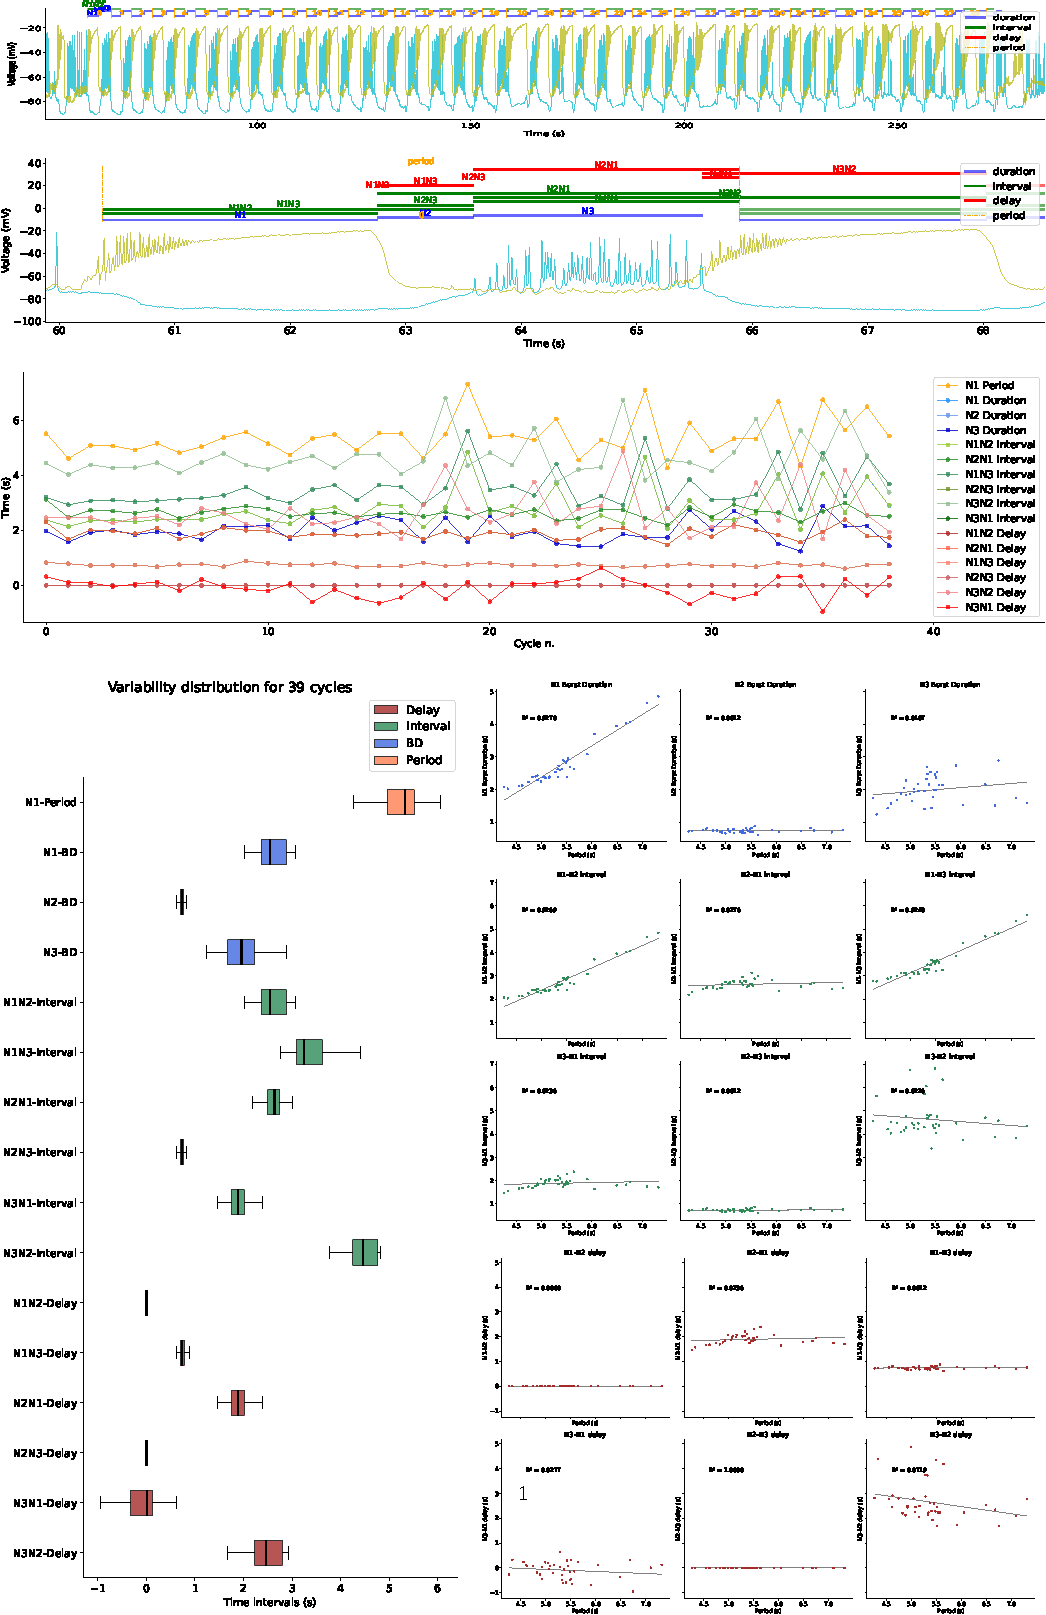
\includegraphics[width=1.1\textwidth]{./invariants/data/SUSSEX/CV1a_driven1/images/3phases/panel_with_intervals.pdf}
	\caption{\textbf{CV1a driven case1}: Panel of intervals distribution and dynamical invariants for the three phases in the CPG under CV1a stimulation.}
	\label{fig:cv1a 1 3phases}
\end{figure}

\begin{figure}[htbp]
	\centering
	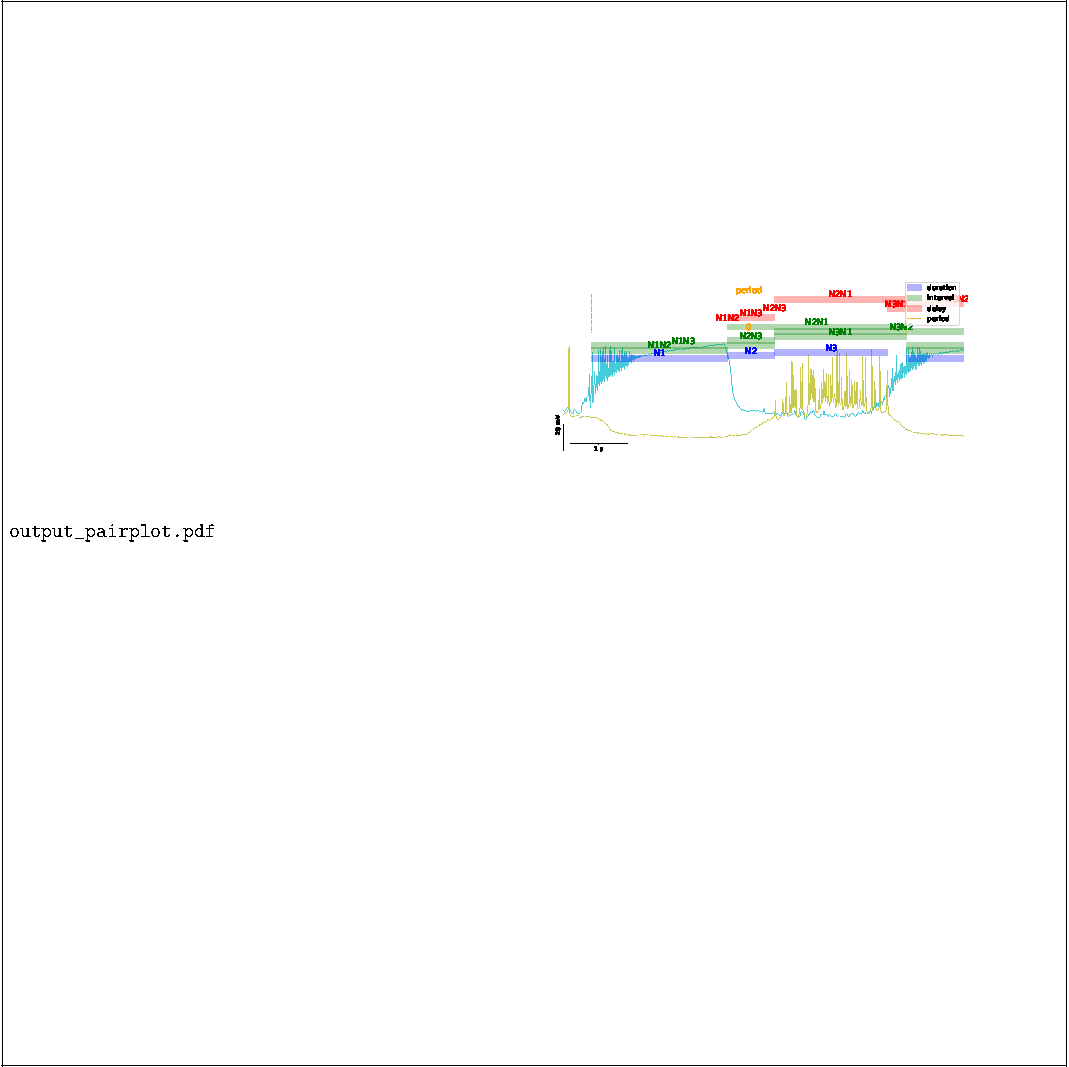
\includegraphics[width=1.1\textwidth]{./invariants/data/SUSSEX/CV1a_driven1/images/3phases/panel_with_pairplot.pdf}
	\caption{\textbf{CV1a driven case1}: Panel of intervals distribution and dynamical invariants for the three phases in the CPG under CV1a stimulation.}
	\label{fig:cv1a 1 3phases pairplot}
\end{figure}

\begin{figure}[htbp]
	\centering
	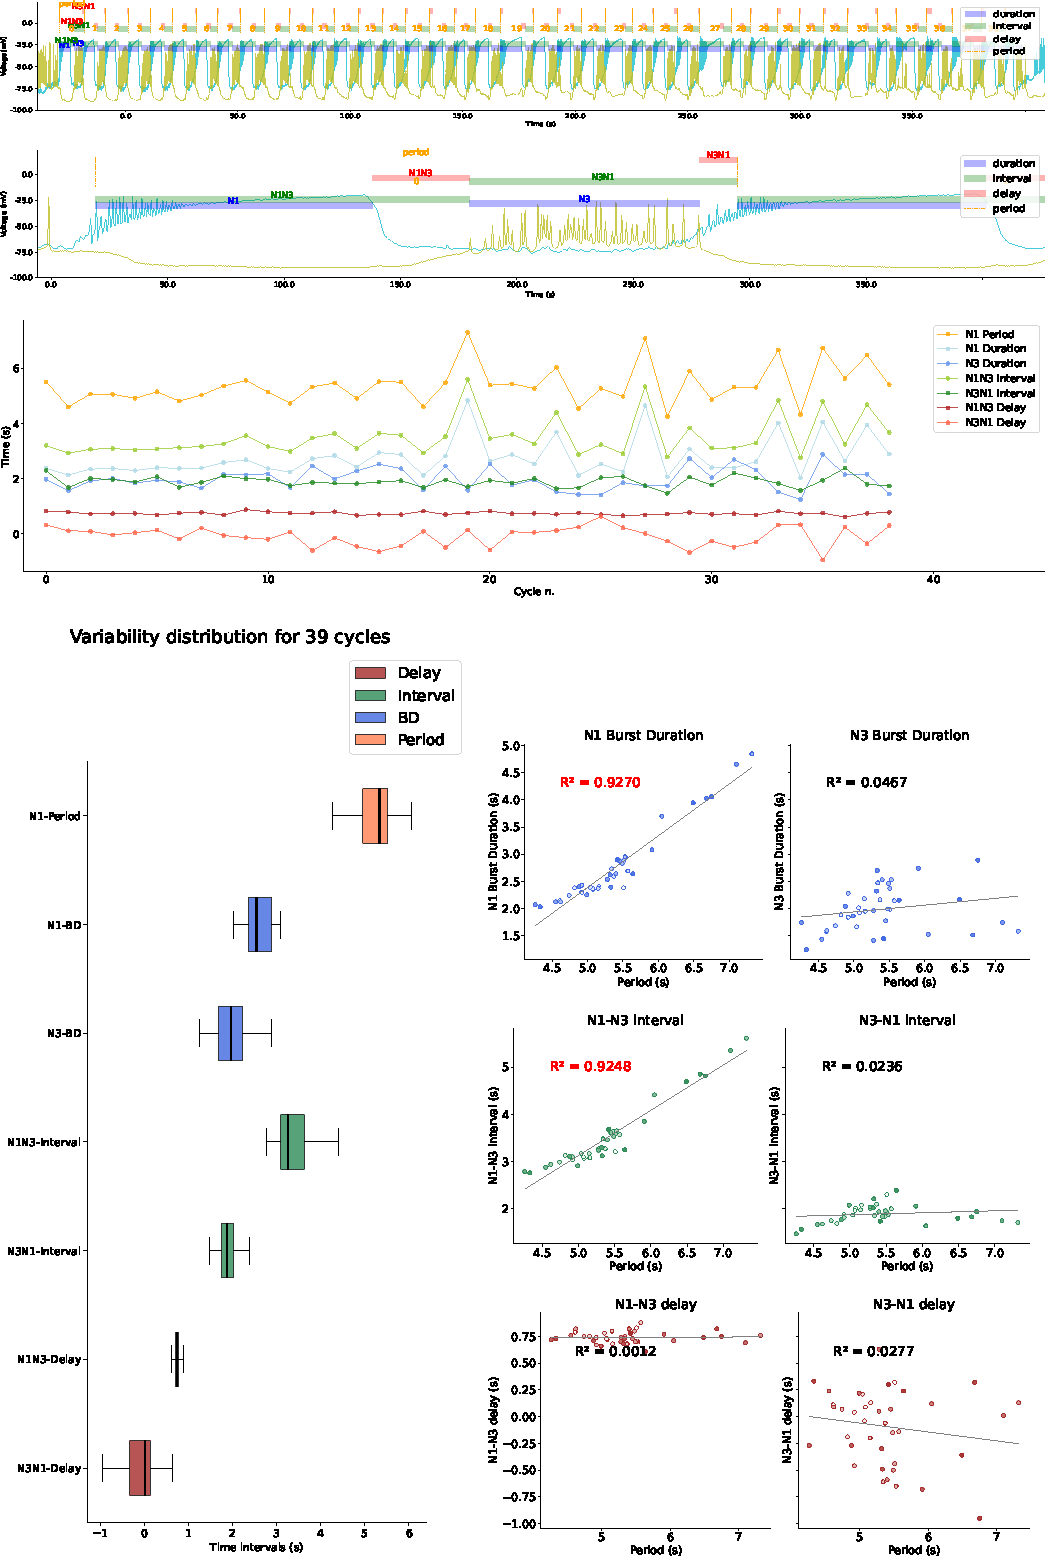
\includegraphics[width=1.1\textwidth]{./invariants/data/SUSSEX/CV1a_driven1/images/2phases/panel_with_intervals.pdf}
	\caption{\textbf{CV1a driven case1}:Panel of intervals distribution and dynamical invariants for the two phases in the CPG under CV1a stimulation.}
	\label{fig:cv1a 1 2phases}
\end{figure}


\begin{figure}[htbp]
	\centering
	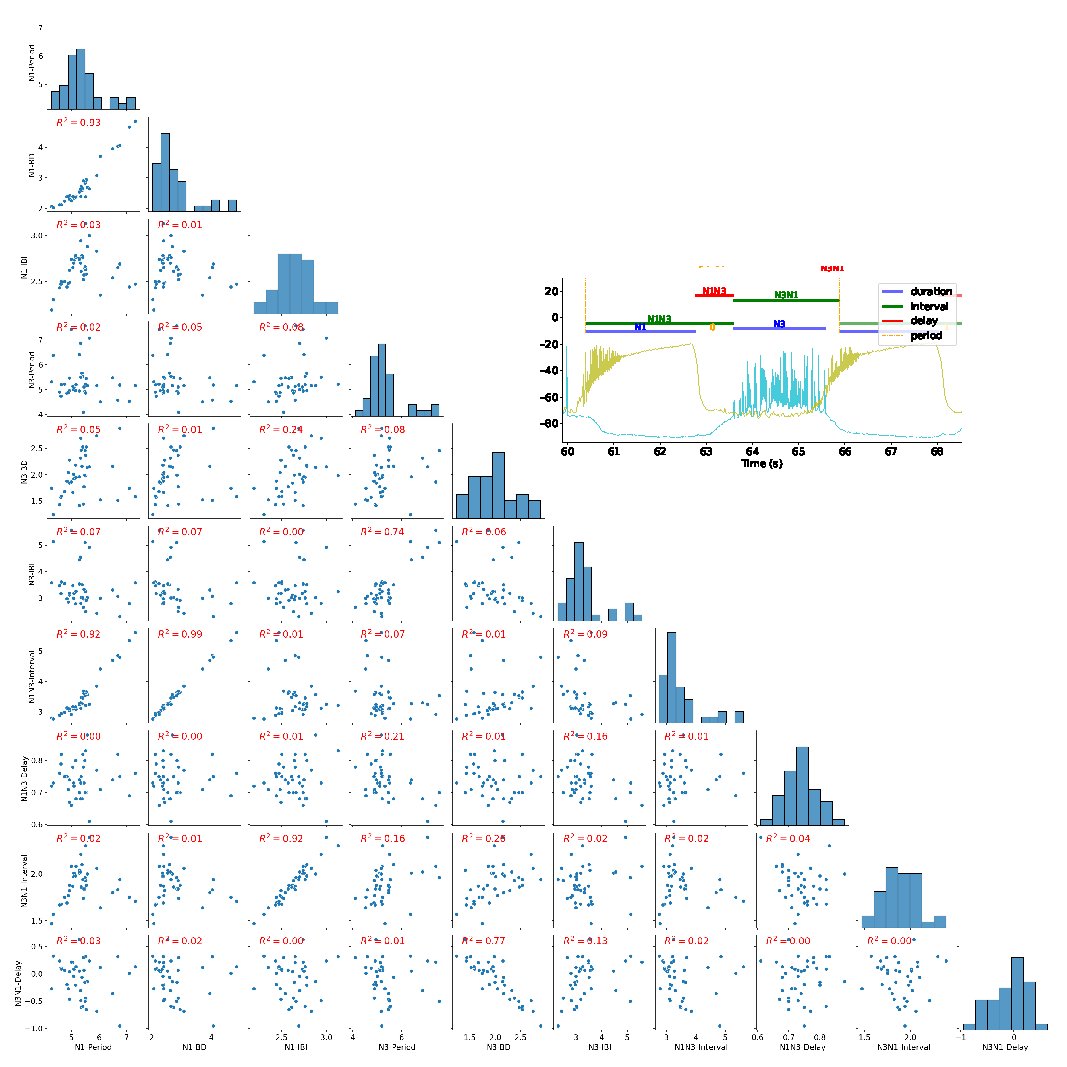
\includegraphics[width=1.1\textwidth]{./invariants/data/SUSSEX/CV1a_driven1/images/2phases/panel_with_pairplot.pdf}
	\caption{\textbf{CV1a driven case1}:Panel of intervals distribution and dynamical invariants for the two phases in the CPG under CV1a stimulation.}
	\label{fig:cv1a 1 2phases pairplot}
\end{figure}



\paragraph{\large{Example 2}}


\begin{figure}[htbp]
	\centering
	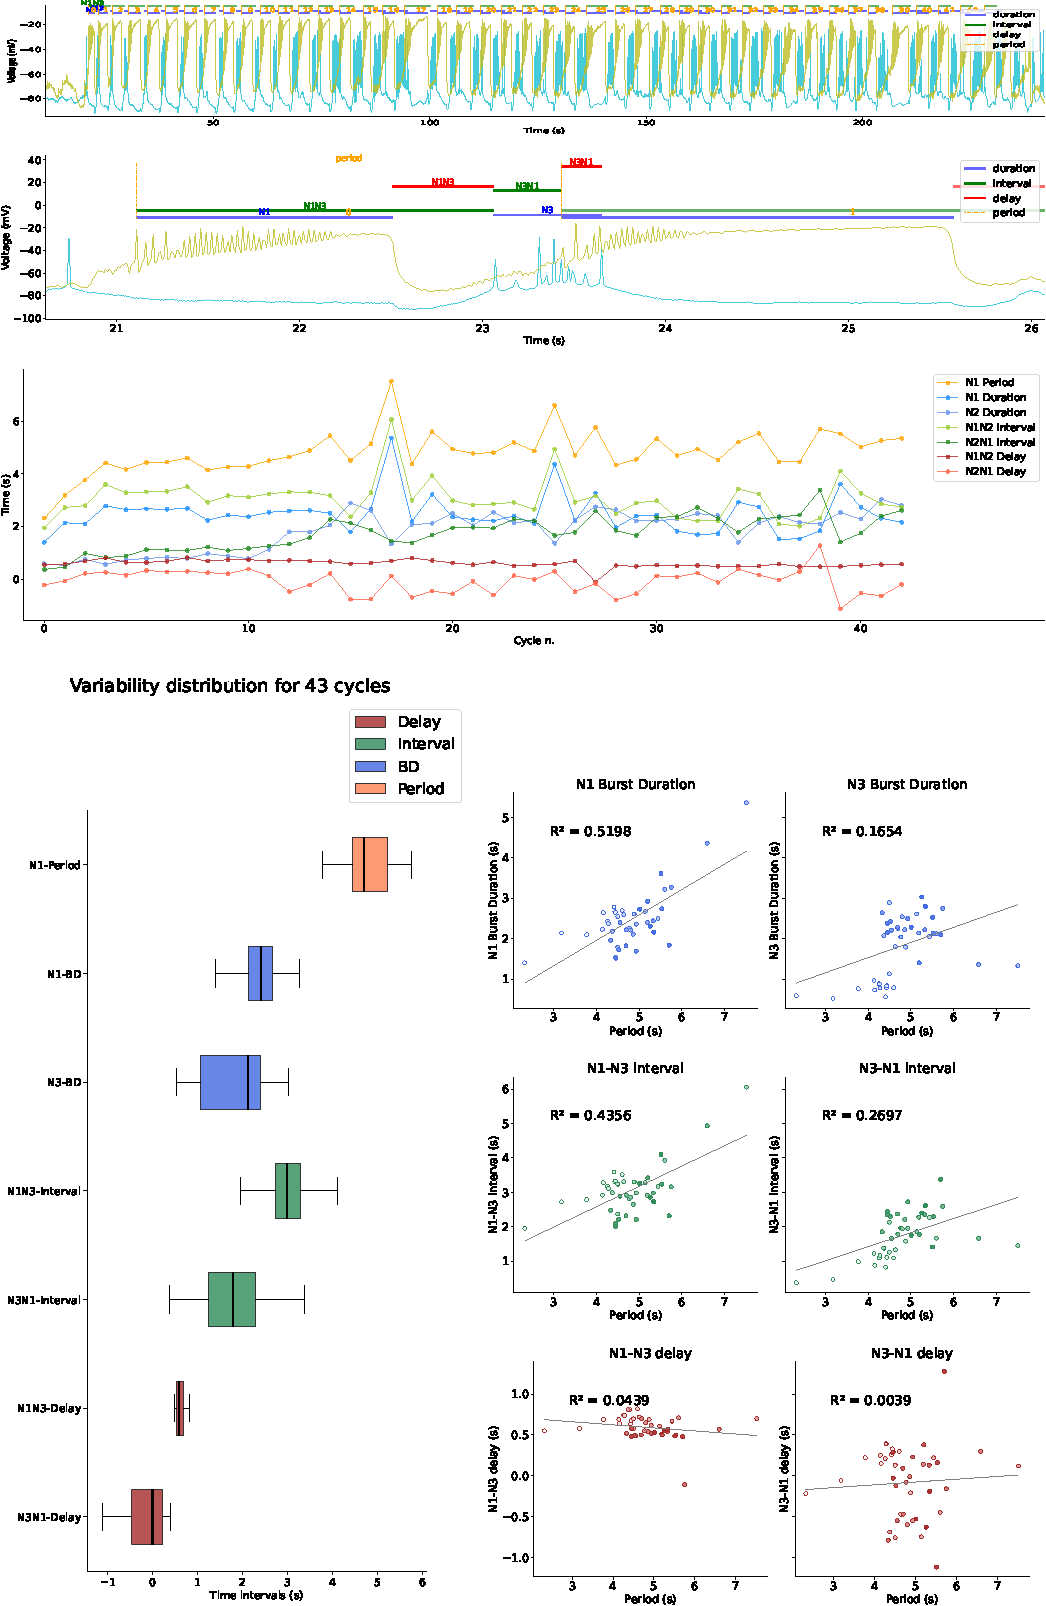
\includegraphics[width=1.1\textwidth]{./invariants/data/SUSSEX/CV1a_driven2/images/panel_with_intervals.pdf}
	
	\caption{\textbf{CV1a driven case2}: Panel of intervals distribution and dynamical invariants for the two phases in the CPG under CV1a stimulation.}
	\label{fig:cv1a 2 2phases}
\end{figure}


\begin{figure}[htbp]
	\centering
	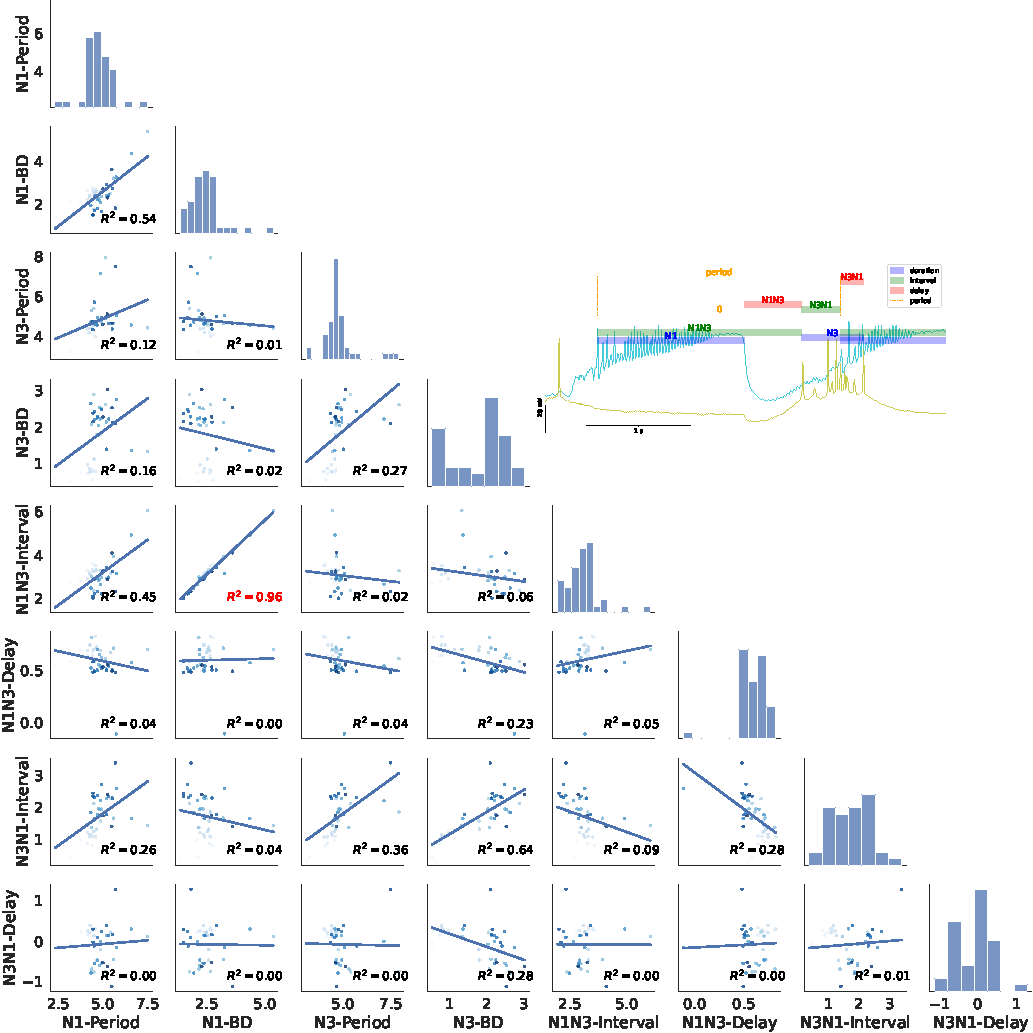
\includegraphics[width=1.1\textwidth]{./invariants/data/SUSSEX/CV1a_driven2/images/panel_with_pairplot.pdf}
	
	\caption{\textbf{CV1a driven case2}: Panel of intervals distribution and dynamical invariants for the two phases in the CPG under CV1a stimulation.}
	\label{fig:cv1a 2 2phases pairplot}
\end{figure}




\paragraph{\large{Example 3}}


\begin{figure}[htbp]
	\centering
	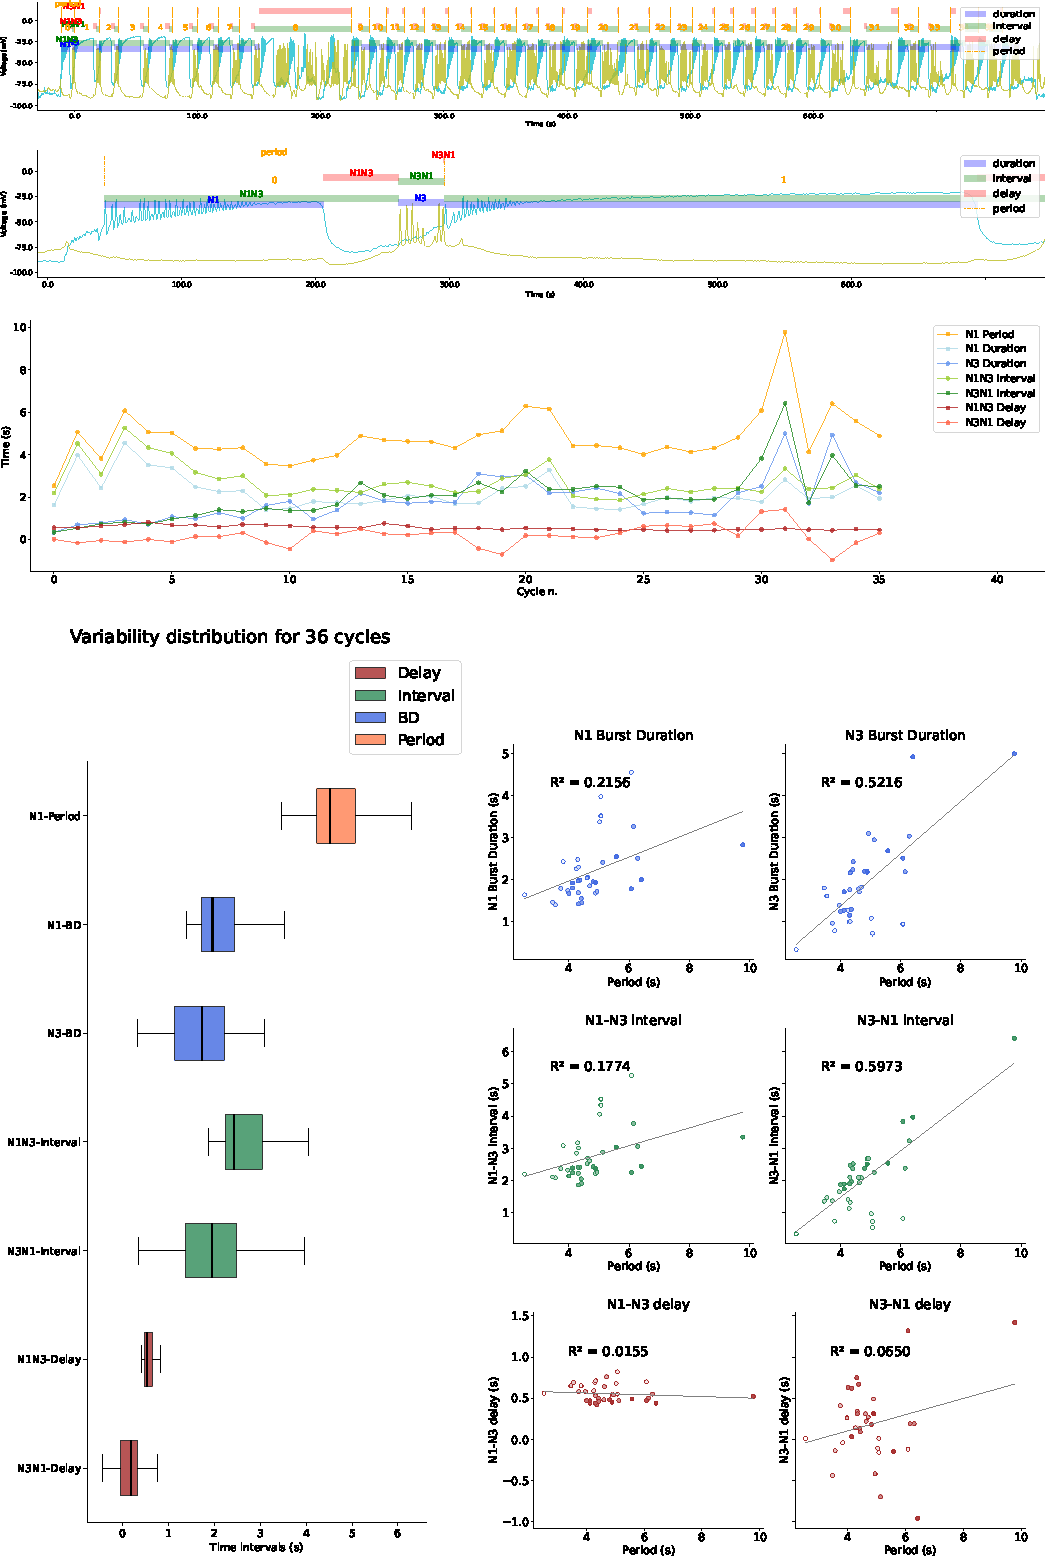
\includegraphics[width=1.1\textwidth]{./invariants/data/SUSSEX/CV1a_driven3/images/panel_with_intervals.pdf}
	\caption{\textbf{CV1a driven case3}: Panel of intervals distribution and dynamical invariants for the two phases in the CPG under CV1a stimulation.}
	\label{fig:cv1a 3 2phases}
\end{figure}



\paragraph{\large{Example 4}}

\begin{figure}[htbp]
	\centering
	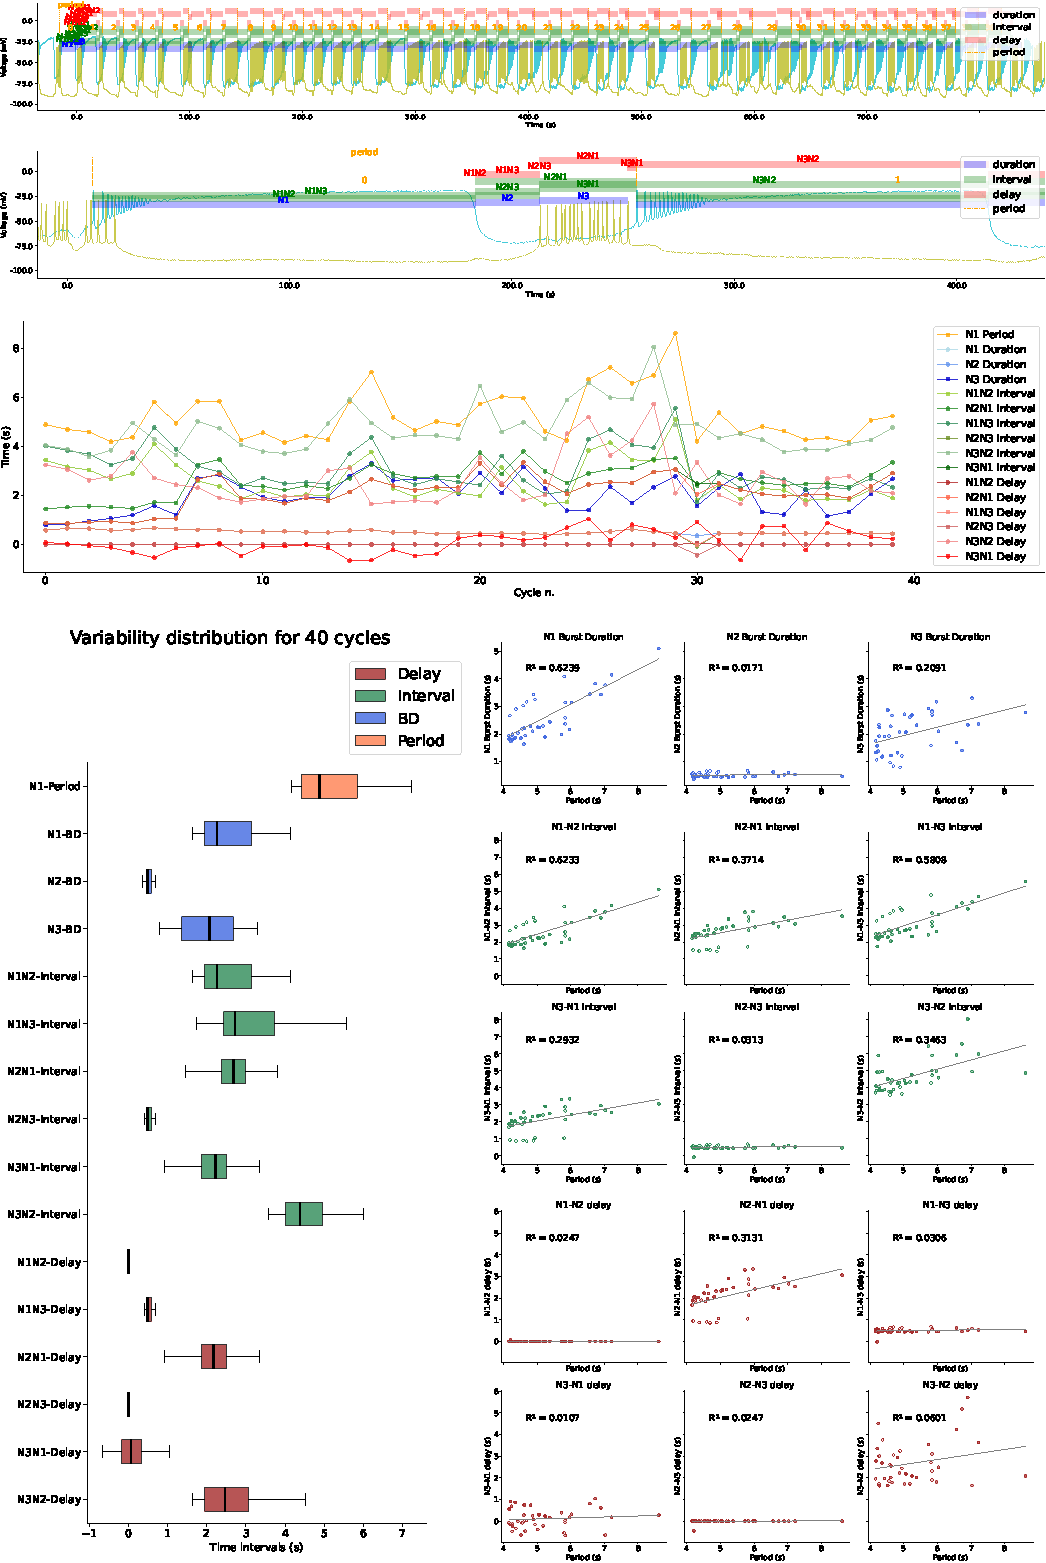
\includegraphics[width=1.1\textwidth]{./invariants/data/SUSSEX/CV1a_driven4/images/3phases/panel_with_intervals.pdf}
	\caption{\textbf{CV1a driven case 4}: Panel of intervals distribution and dynamical invariants for the three phases in the CPG under CV1a stimulation.}
	\label{fig:cv1a 4 3phases}
\end{figure}

\begin{figure}[htbp]
	\centering
	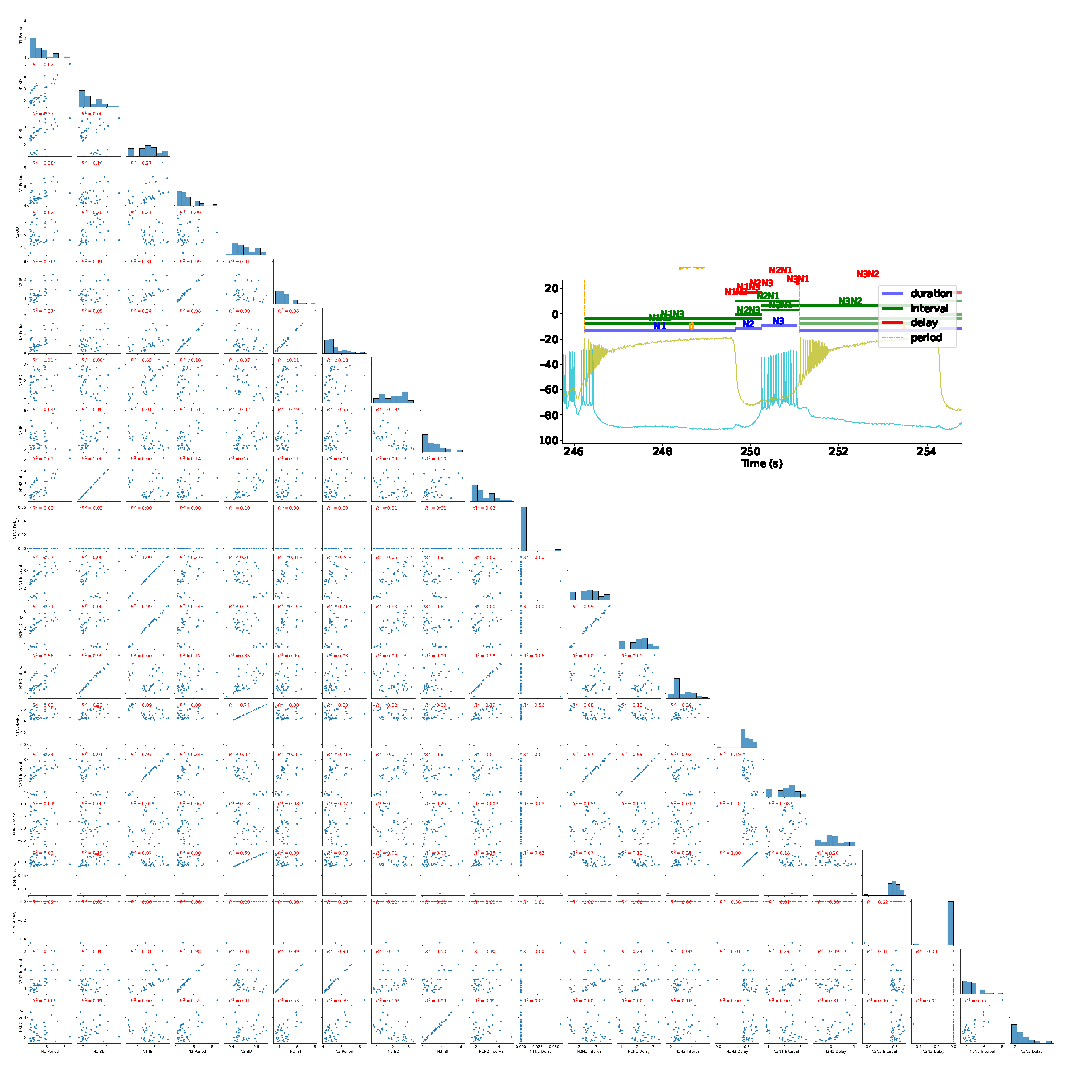
\includegraphics[width=1.1\textwidth]{./invariants/data/SUSSEX/CV1a_driven4/images/3phases/panel_with_pairplot.pdf}
	\caption{\textbf{CV1a driven case 4}: Panel of intervals distribution and dynamical invariants for the three phases in the CPG under CV1a stimulation.}
	\label{fig:cv1a 4 3phases pairplot}
\end{figure}

\begin{figure}[htbp]
	\centering
	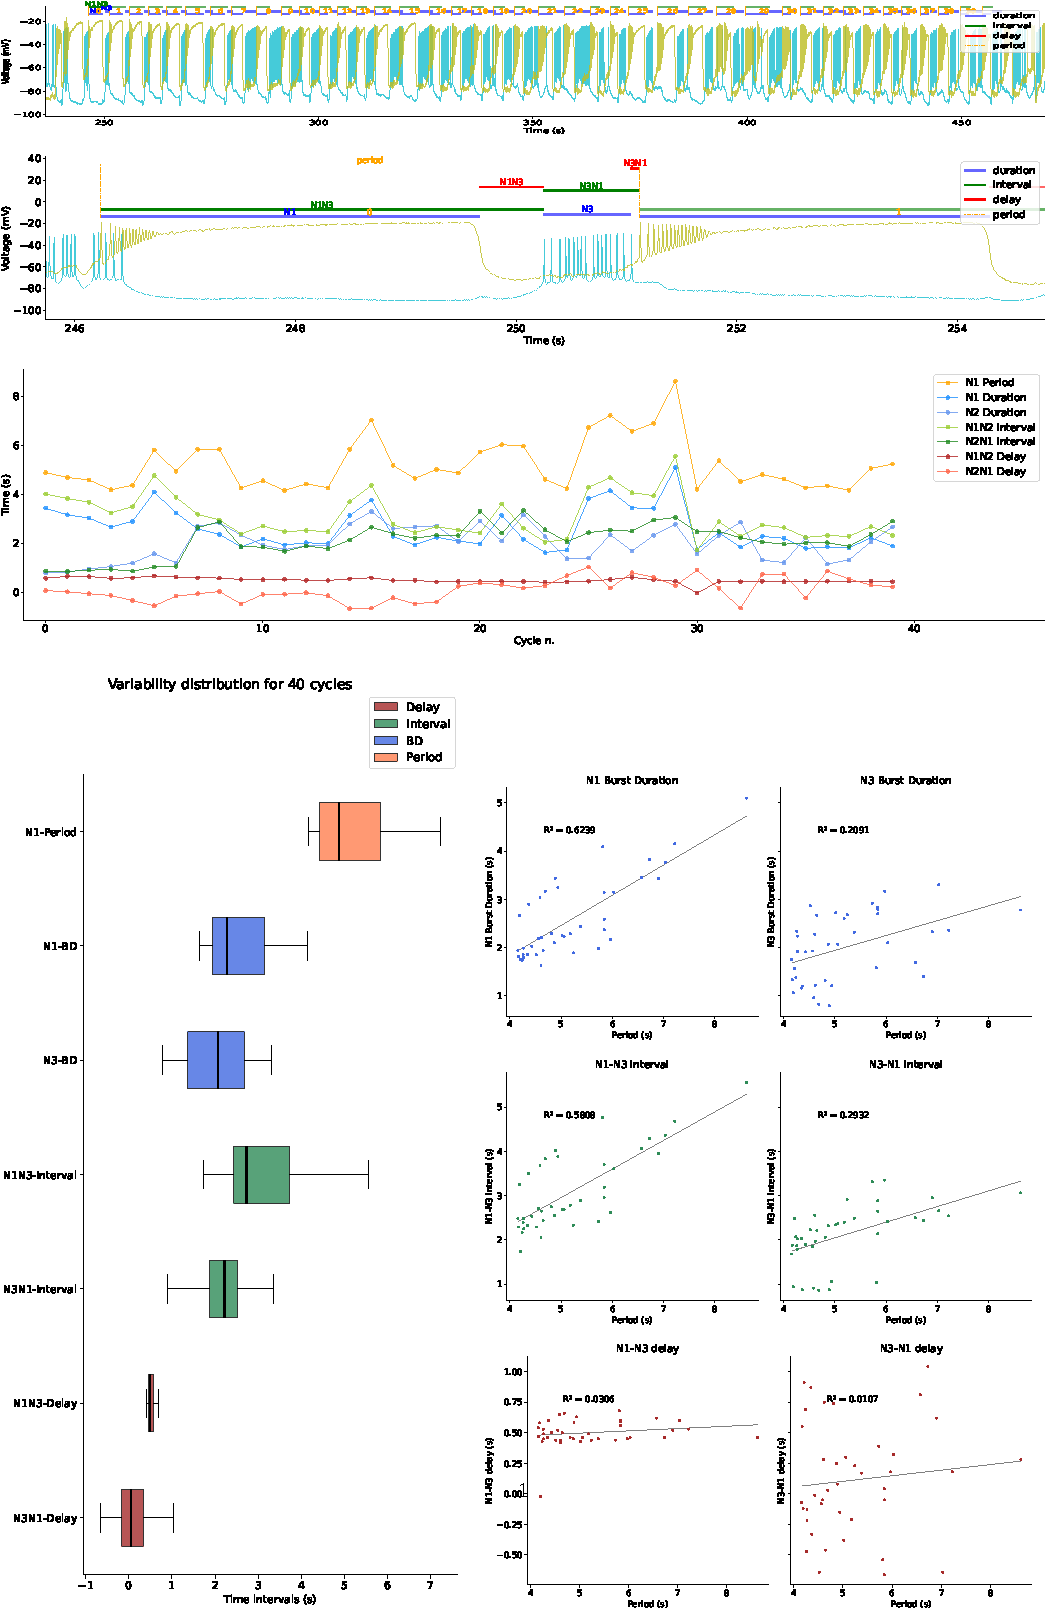
\includegraphics[width=1.1\textwidth]{./invariants/data/SUSSEX/CV1a_driven4/images/2phases/panel_with_intervals.pdf}
	\caption{\textbf{CV1a driven case4}: Panel of intervals distribution and dynamical invariants for the two phases in the CPG under CV1a stimulation.}
	\label{fig:cv1a 4 2phases}
\end{figure}

\begin{figure}[htbp]
	\centering
	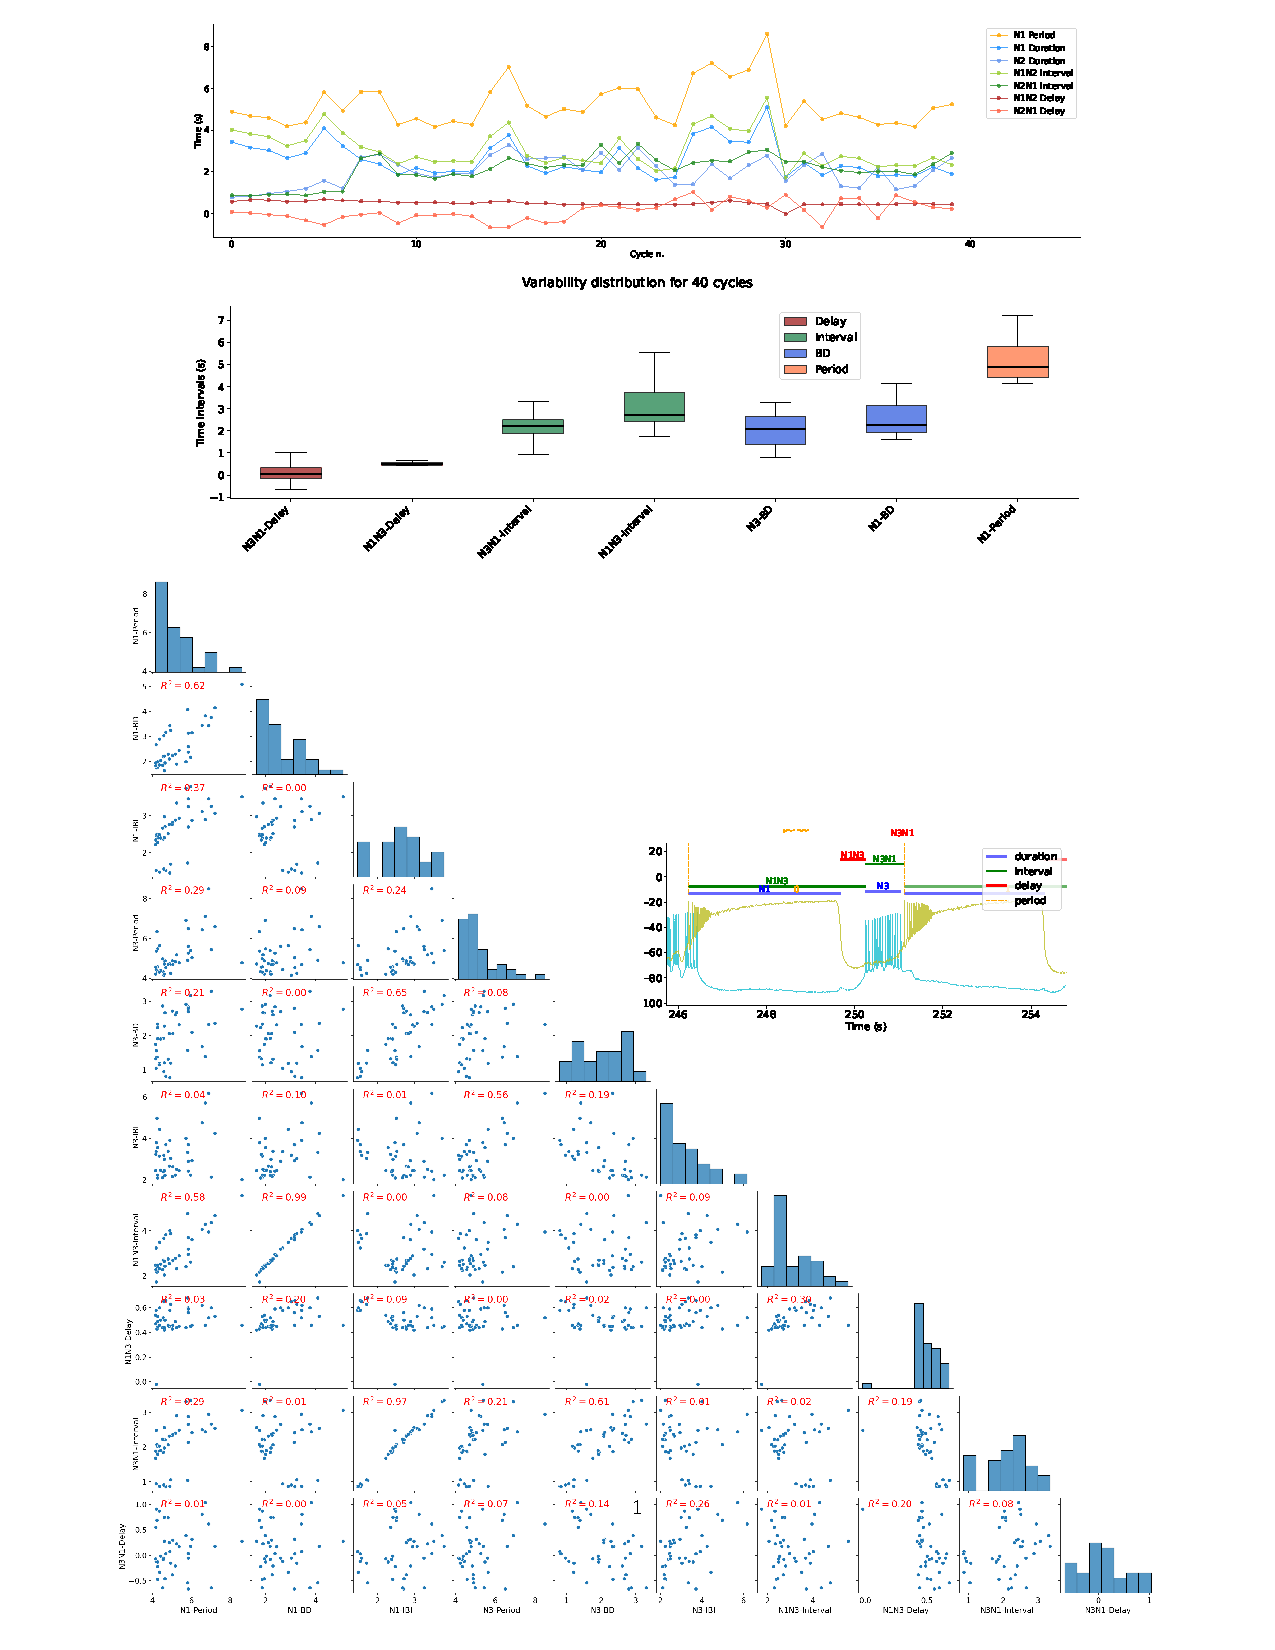
\includegraphics[width=1.1\textwidth]{./invariants/data/SUSSEX/CV1a_driven4/images/2phases/panel_with_pairplot.pdf}
	\caption{\textbf{CV1a driven case4}: Panel of intervals distribution and dynamical invariants for the two phases in the CPG under CV1a stimulation.}
	\label{fig:cv1a 4 2phases pairplot}
\end{figure}


\begin{figure}
	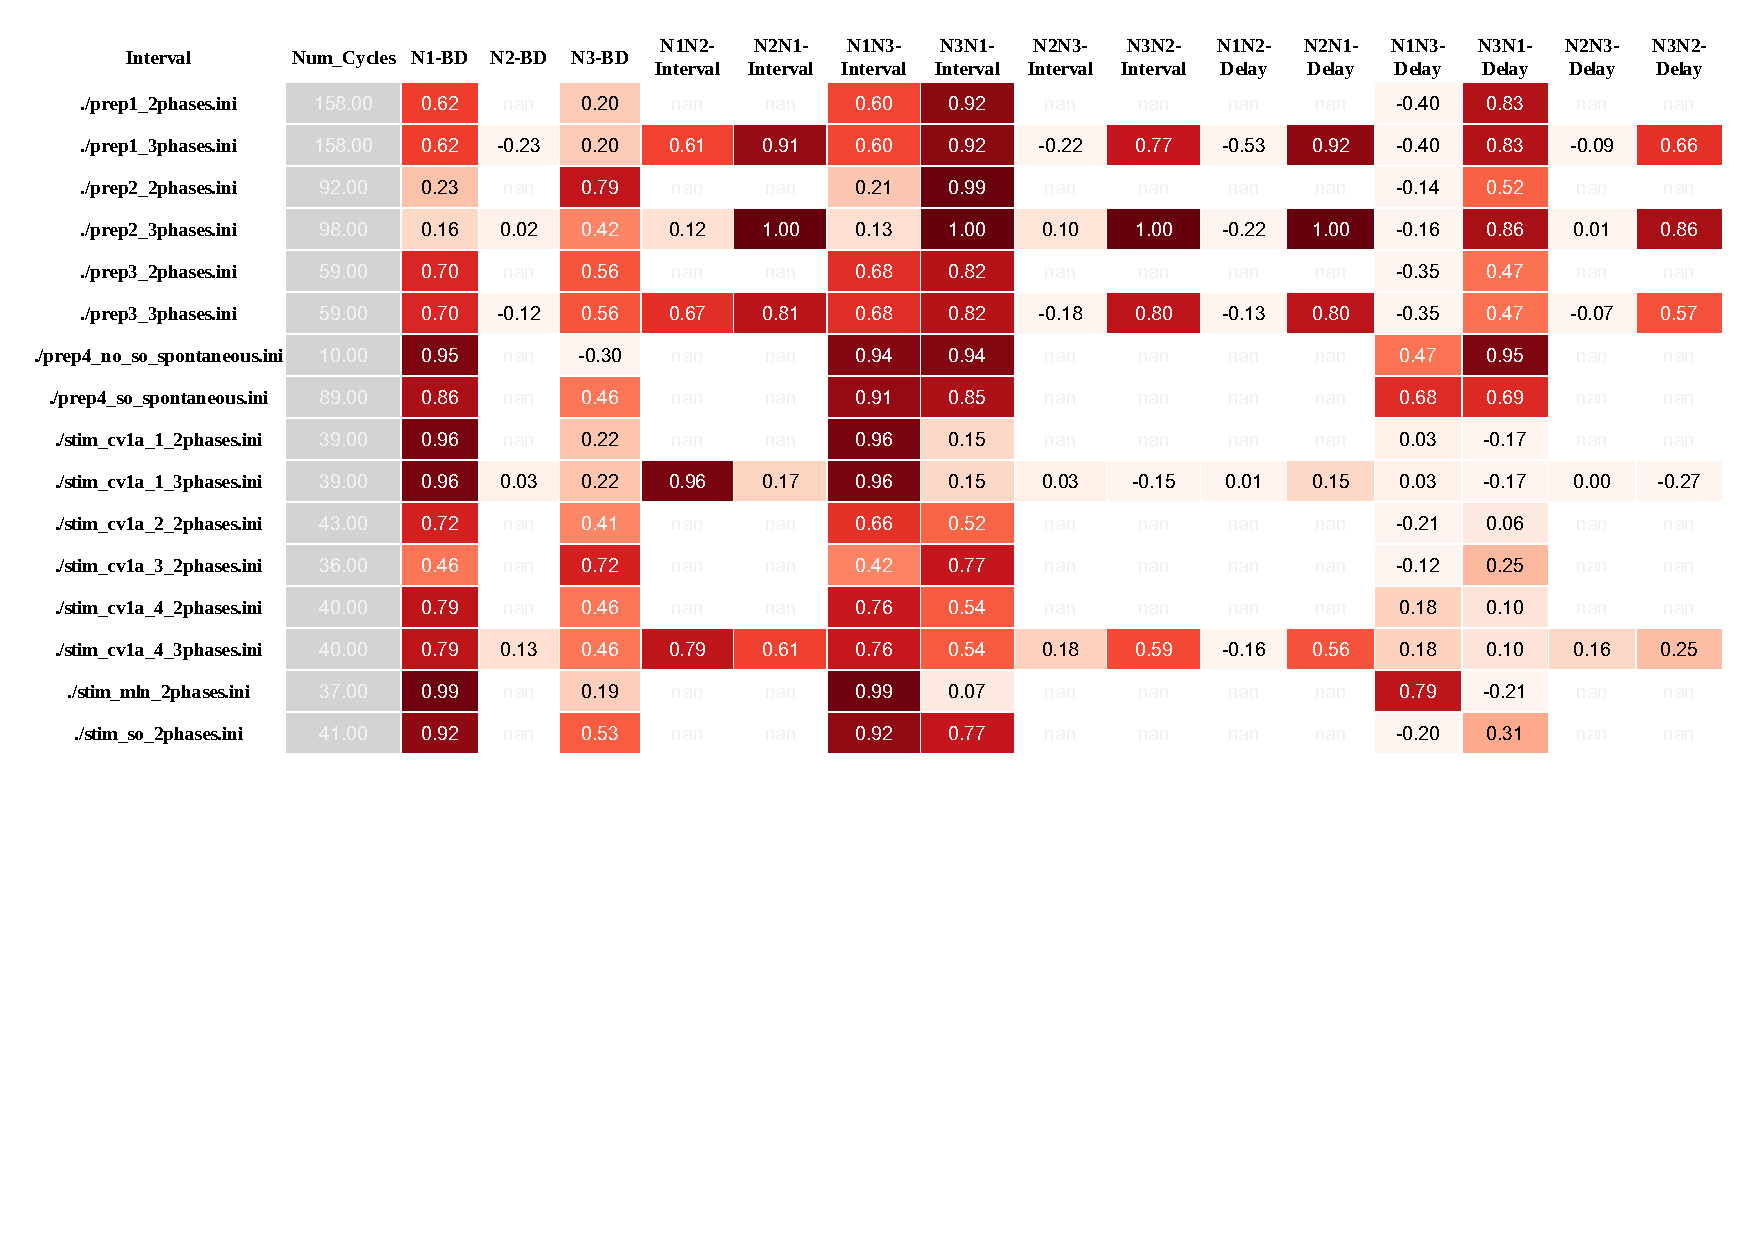
\includegraphics[width=\textwidth]{./invariants/styled_table_invariants.pdf}
	\caption{Table of $R^2$ values for the linear regression between the period and each interval for all experimental recordings showed in this section.}
	\label{fig:R2 table}
\end{figure}



